\documentclass{article}
\usepackage{graphicx}
\graphicspath{ {../graphs/} }
\usepackage{geometry}
\geometry{a4paper, portrait, margin=1.0in}
\usepackage{booktabs}
\title{Computational Physics Project A\\Finite Differential Methods (FDMs) for solving Ordinary Differential Equations(ODEs) } % Title

\author{Robert \textsc{Stein}} % Author name

\date{\today} % Date for the report

\begin{document}

\maketitle % Insert the title, author and date
\section{Introduction}
Finite Differential Methods (FDMs) are methods to solve Odinary Differential Equations (ODEs) in discrete steps. When applied to a physical system, their stability can be assessed by checking if solutions obey the law of energy conservation. In both damped and undamped systems, the system energy must \textbf{never} increase. 

In the strictest test, we could define a stable system as one in which the total energy of the system never exceeds the initial energy of the system. However, an undamped system with a slightly fluctuating energy could still have a stable average energy. Such undamped systems will nonetheless fail to meet the stability criteria, so an additional threshold of tolerance, requiring the step energy to not exceed 100.1\% of the initial energy, is implemented.

\section{Single Pendulum}
The single pendulum is a simple system useful for comparing FDMs. For a pendulum of mass $m_{1}$, we define $\theta$ as the angle between the pendulum and the verticle. The dynamics are determined by the equation of motion:

\[ \frac{d^{2}\theta}{dt^{2}} = - \frac{g}{l} \sin(\theta) - \frac{D}{ml} \frac{d\theta}{dt} \]

A transformation of this equation is described in the Appendix, along with a derivation of the pendulum energy. With the energy value, we can measure the stability of solutions.
\subsection{Finite Differential Methods}
Four FDMs were chosen for analysis, namely the Explicit Euler and Implicit Euler methods, as well as the Leapfrog method and the Runge-Kutta 4 method. A brief description of each is given in the Appendix. The results of the undamped and damped simulations can be found in Figures \ref{fig:singleundampedenergy} and \ref{fig:singledampedenergy} respectively. 

\begin{figure}
\begin{center}
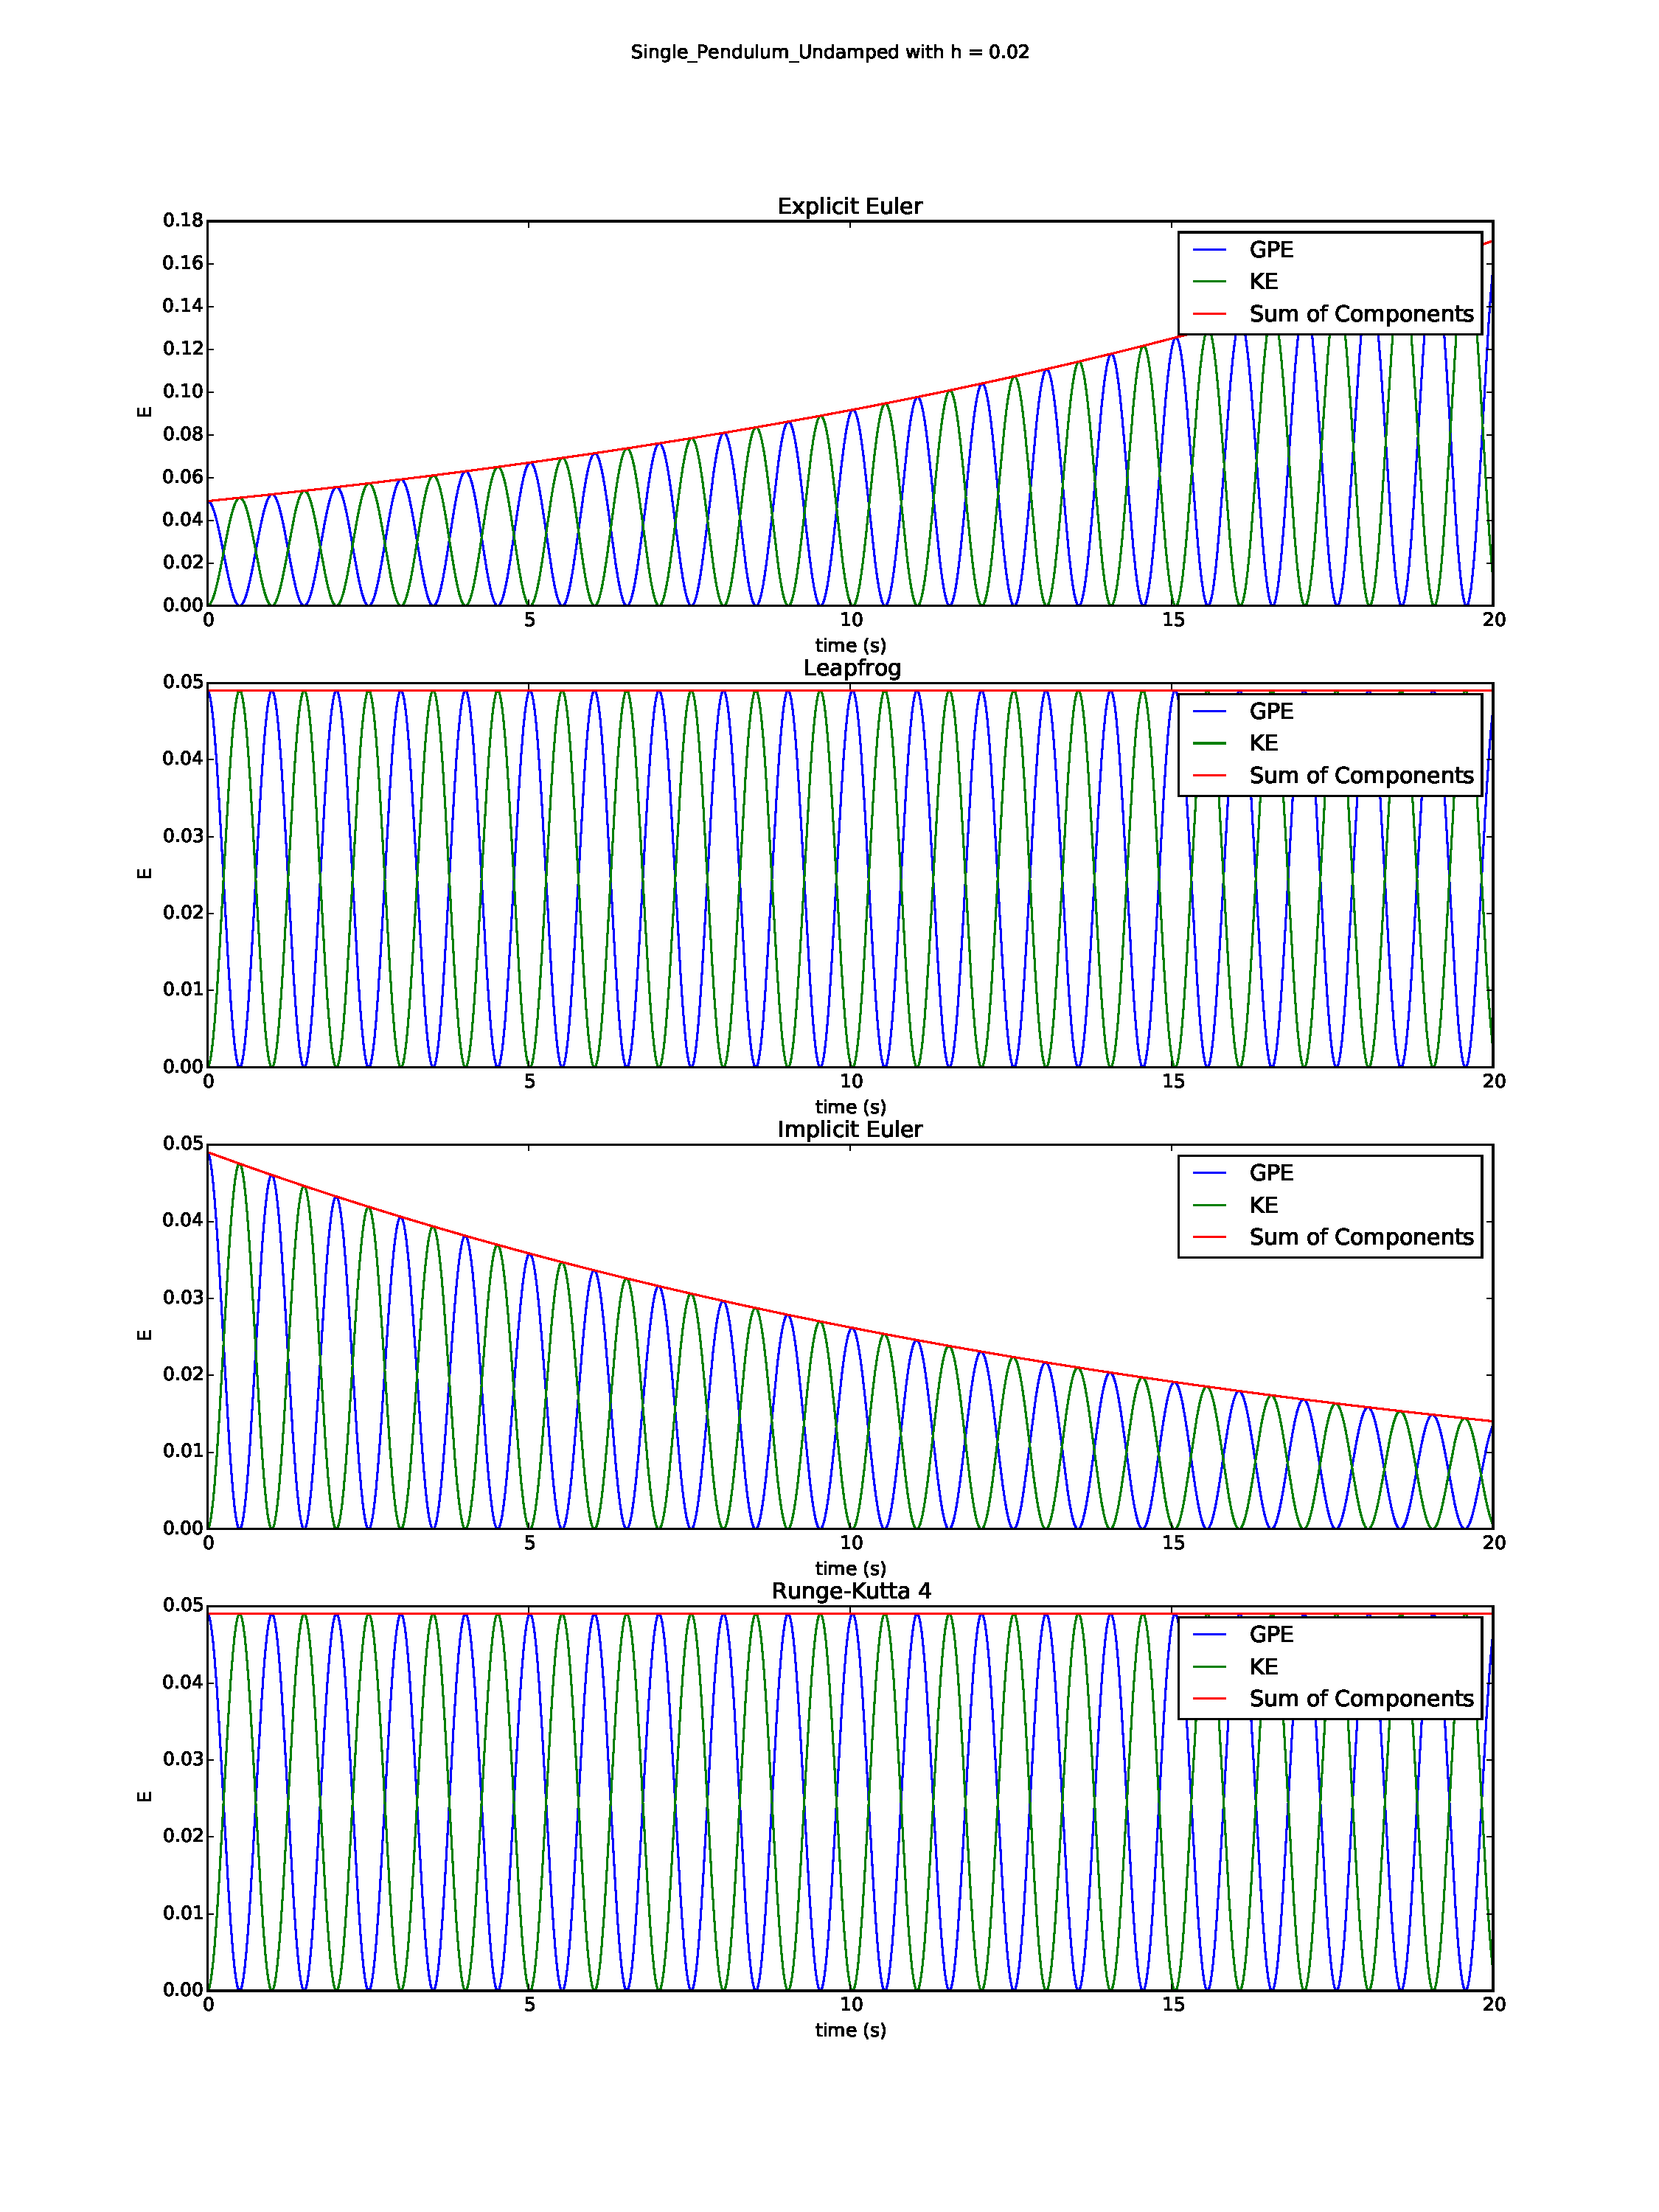
\includegraphics[height=0.9\textheight]{Single_Pendulum_Undamped_Energy_Components}
\caption{The solutions for an undamped single pendulum with $\hat{D}=0$. }
\label{fig:singleundampedenergy}
\end{center}
\end{figure}

\begin{figure}
\begin{center}
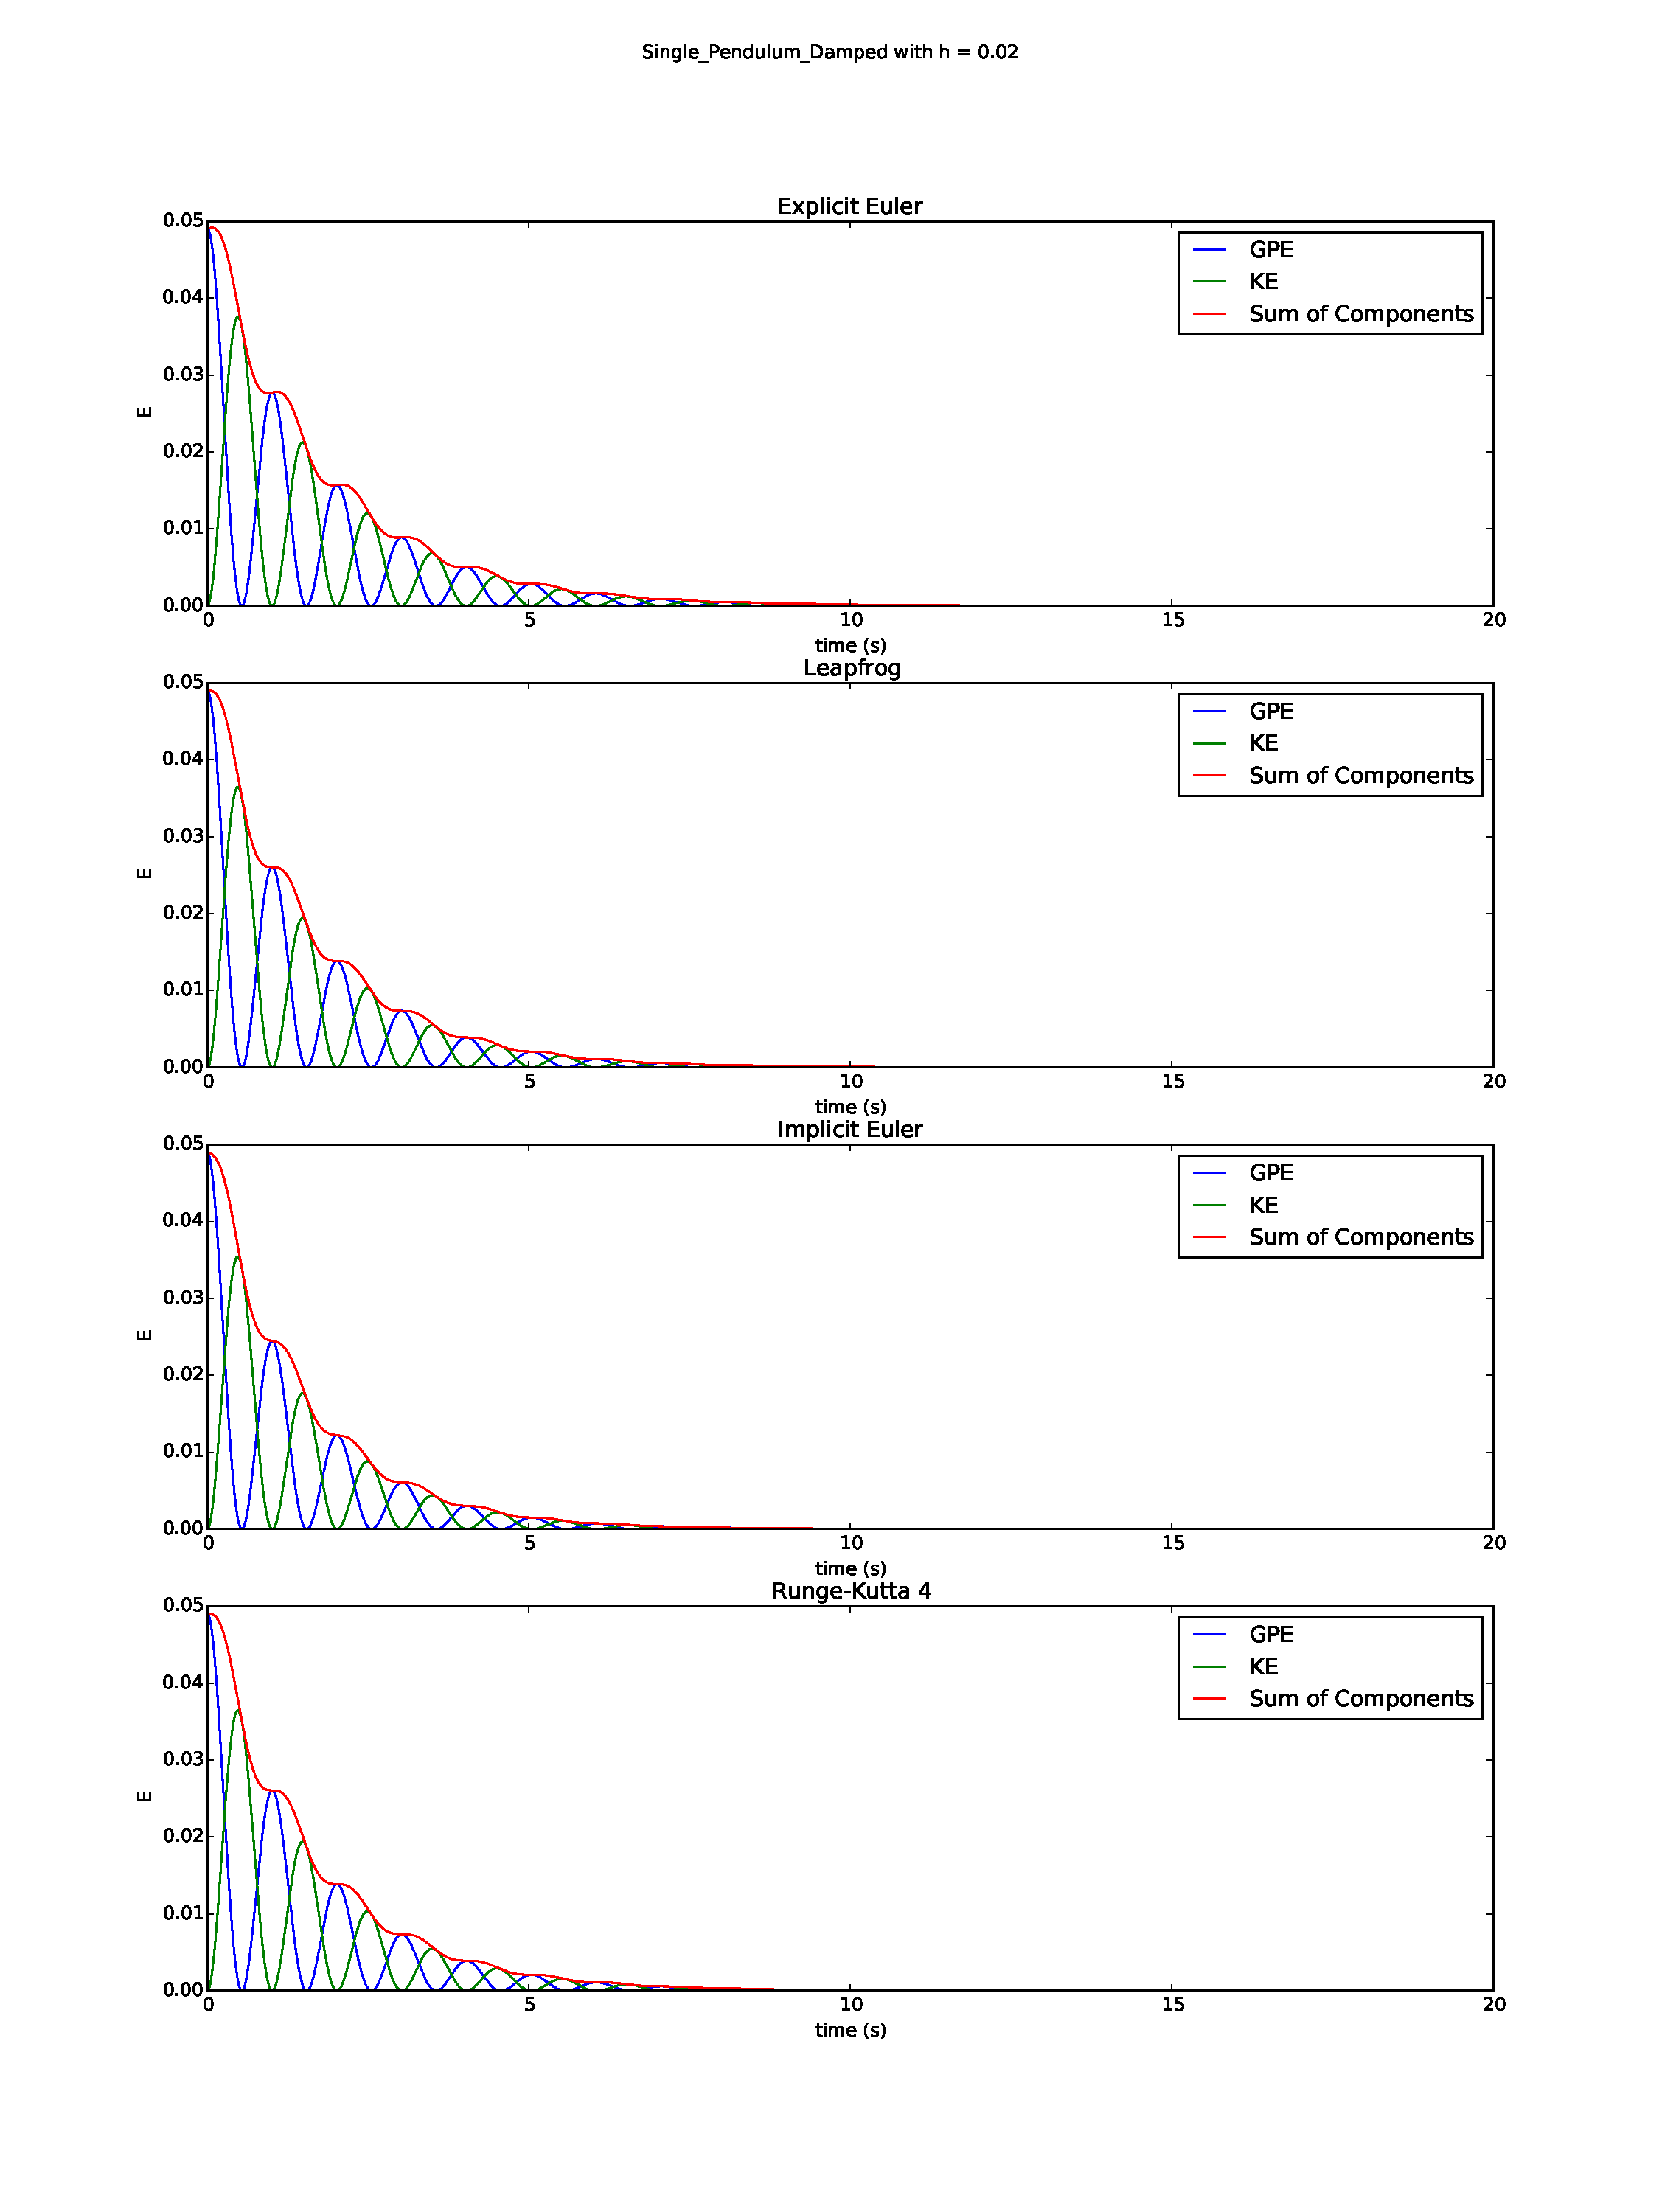
\includegraphics[height=0.9\textheight]{Single_Pendulum_Damped_Energy_Components}
\caption{The solutions for a damped single pendulum with $\hat{D}=0.2$. The system energy is flat when all energy is GPE, because the pendulum is motionless and thus there is no damping. However, as KE is non-zero, damping reduces the total system energy.}
\label{fig:singledampedenergy}
\end{center}
\end{figure}

In the case of the undamped pendulum, we can explore the behaviour of a system with non-decaying energy. The Explicit Euler method is particularly unsuited to this type of ODE, with a tendency for undamped oscillations to increase exponentially. Similarly, the Implicit Euler method has a clear tendency for oscillations to decrease exponentially. In contrast, both the Leapfrog and Runge-Kutta methods give the expected stable, constant energies.

However, for the damped pendulum, the Leapfrog method is only stable over shorter time periods. A sufficiently small stepsize h=0.02 leads to a convergence of all 4 methods on one solution, but given time the Leapfrog solution subsequently diverges and the oscillations begin to increase exponentially. In addition, the Explicit Euler method converges slowly and is unstable by our criteria. The Runga-Kutta and Implicit Euler methods are both stable for this case, although the Implicit Euler solution decays more quickly.

\subsection{Comparison of Damped and Undamped Simulations}
We can directly see the impact of the solution stability by examining a graph of the value of $\theta$. It is clear in Figure \ref{fig:singleundampedtheta} that for the undamped case, the solutions begin to diverge over time, mirroring the energy divergence. For the damped case in Figure \ref{fig:singledampedtheta}, Explicit Euler is still unstable for the given stepsize. The other three FDMs produced stable solutions for the given stepsize and time period.

\begin{figure}
\begin{center}
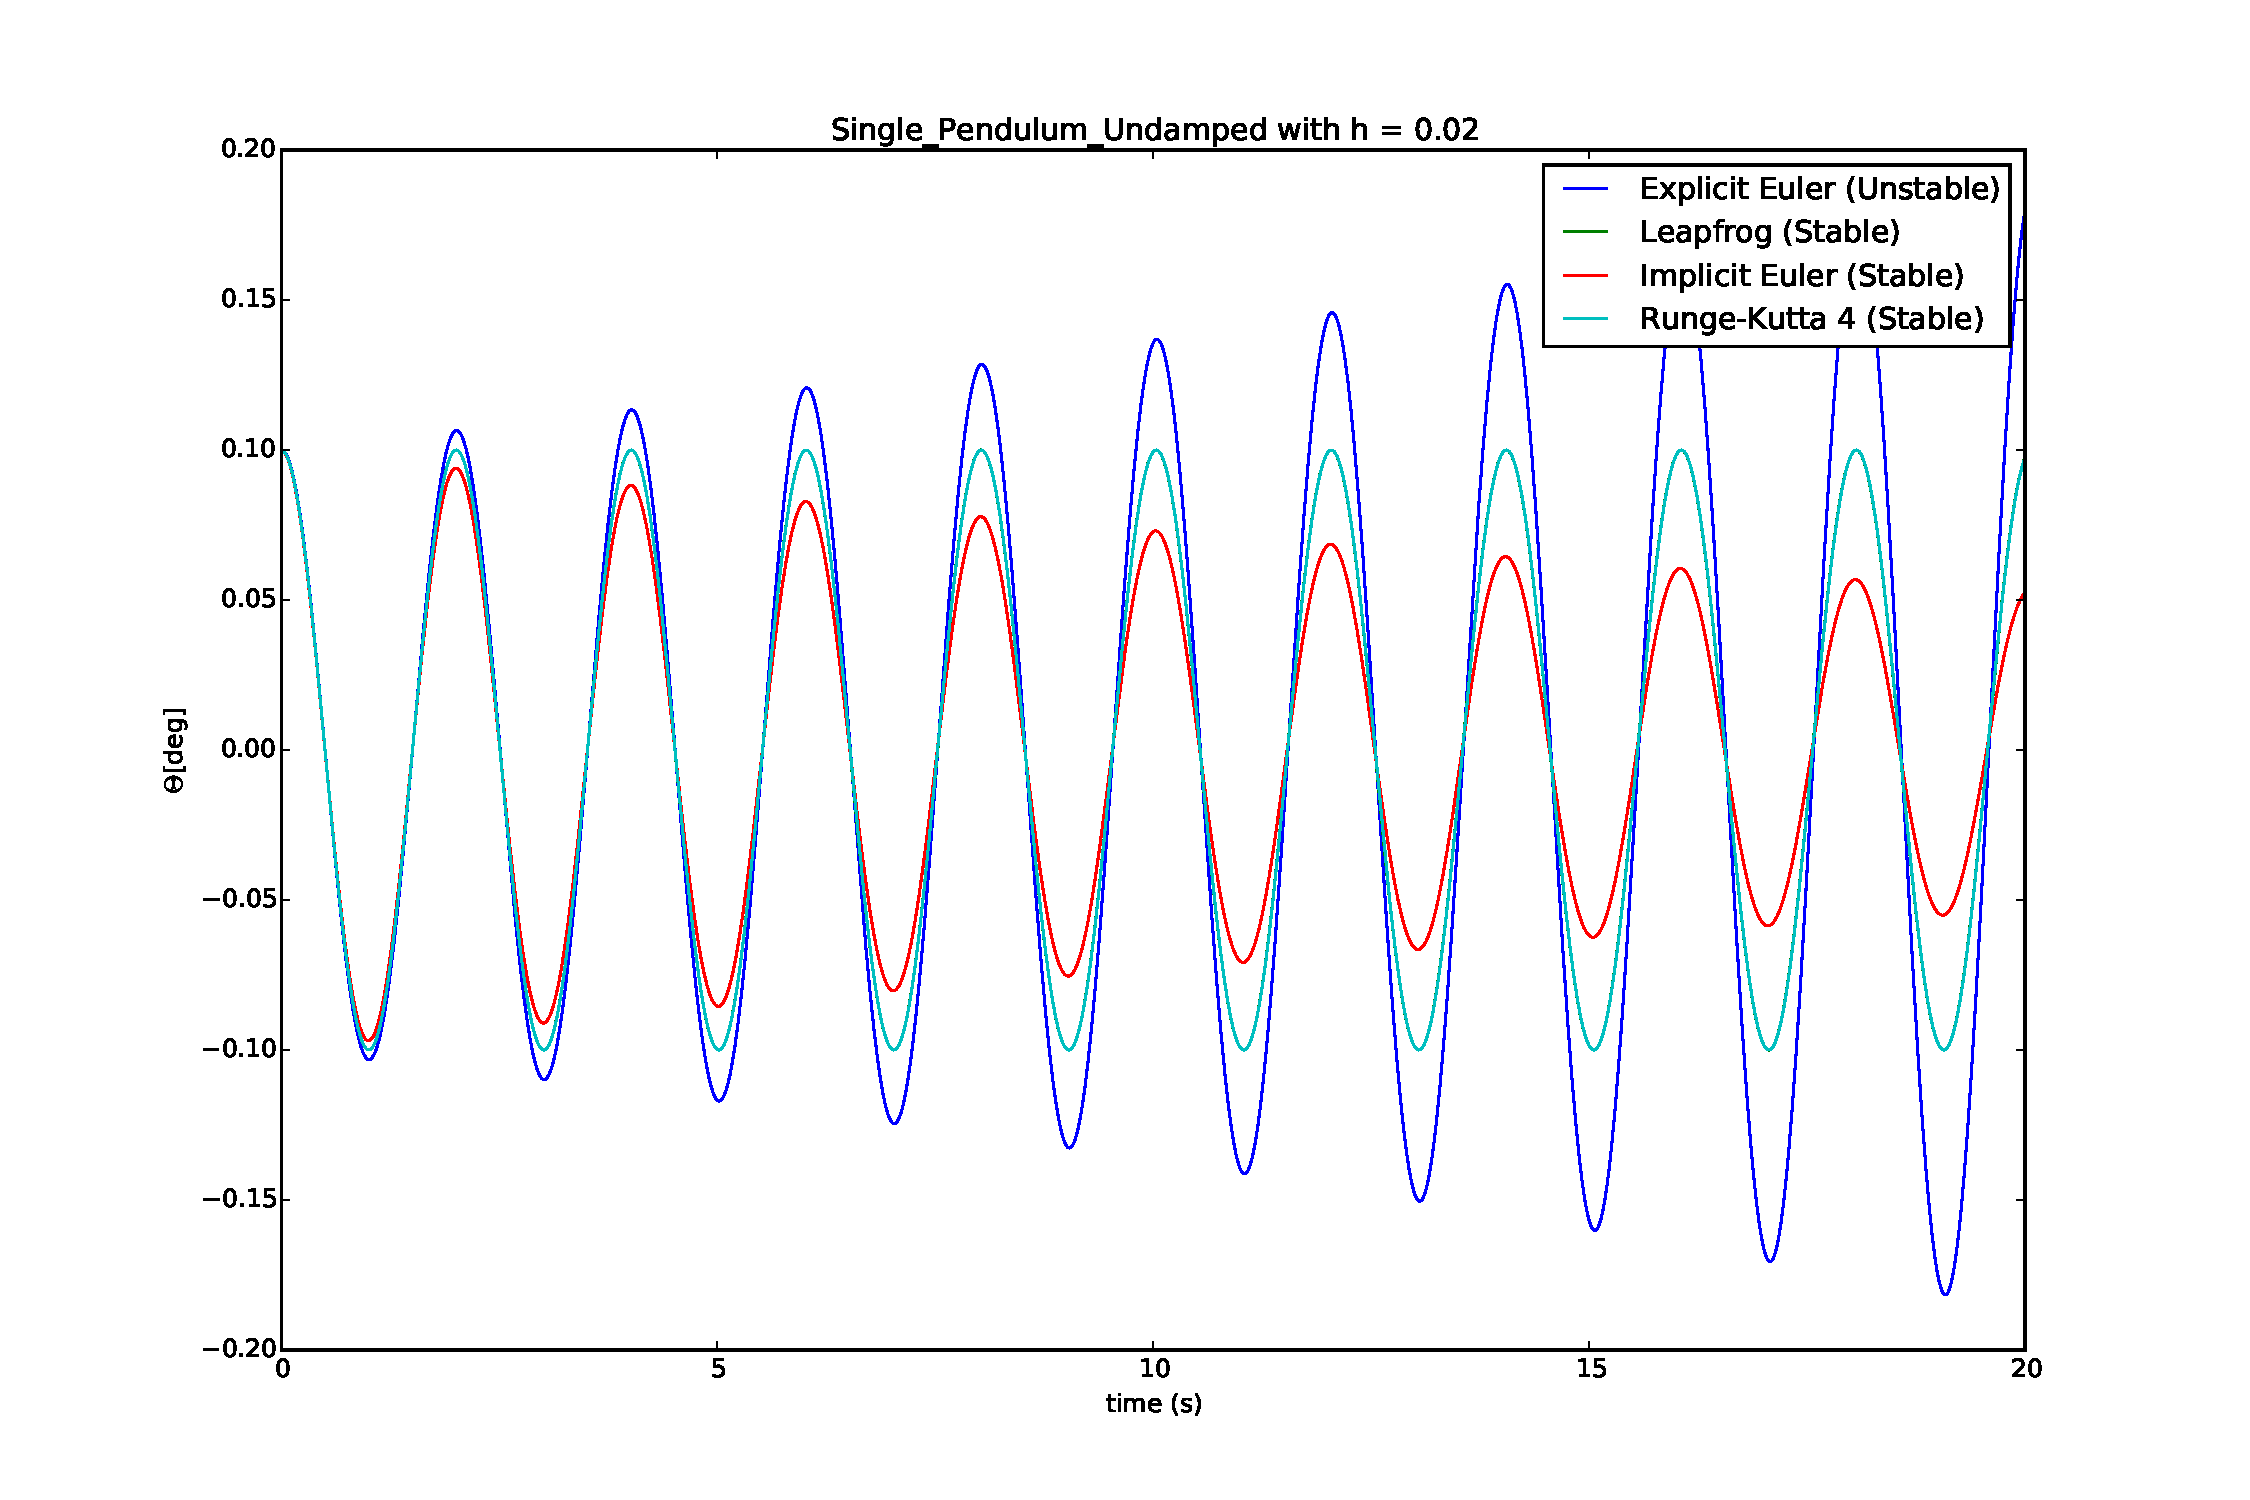
\includegraphics[width=0.9\textwidth]{Single_Pendulum_Undamped_Theta}
\caption{The solutions for an undamped single pendulum with $\hat{D}=0$. }
\label{fig:singleundampedtheta}
\end{center}
\end{figure}

\begin{figure}
\begin{center}
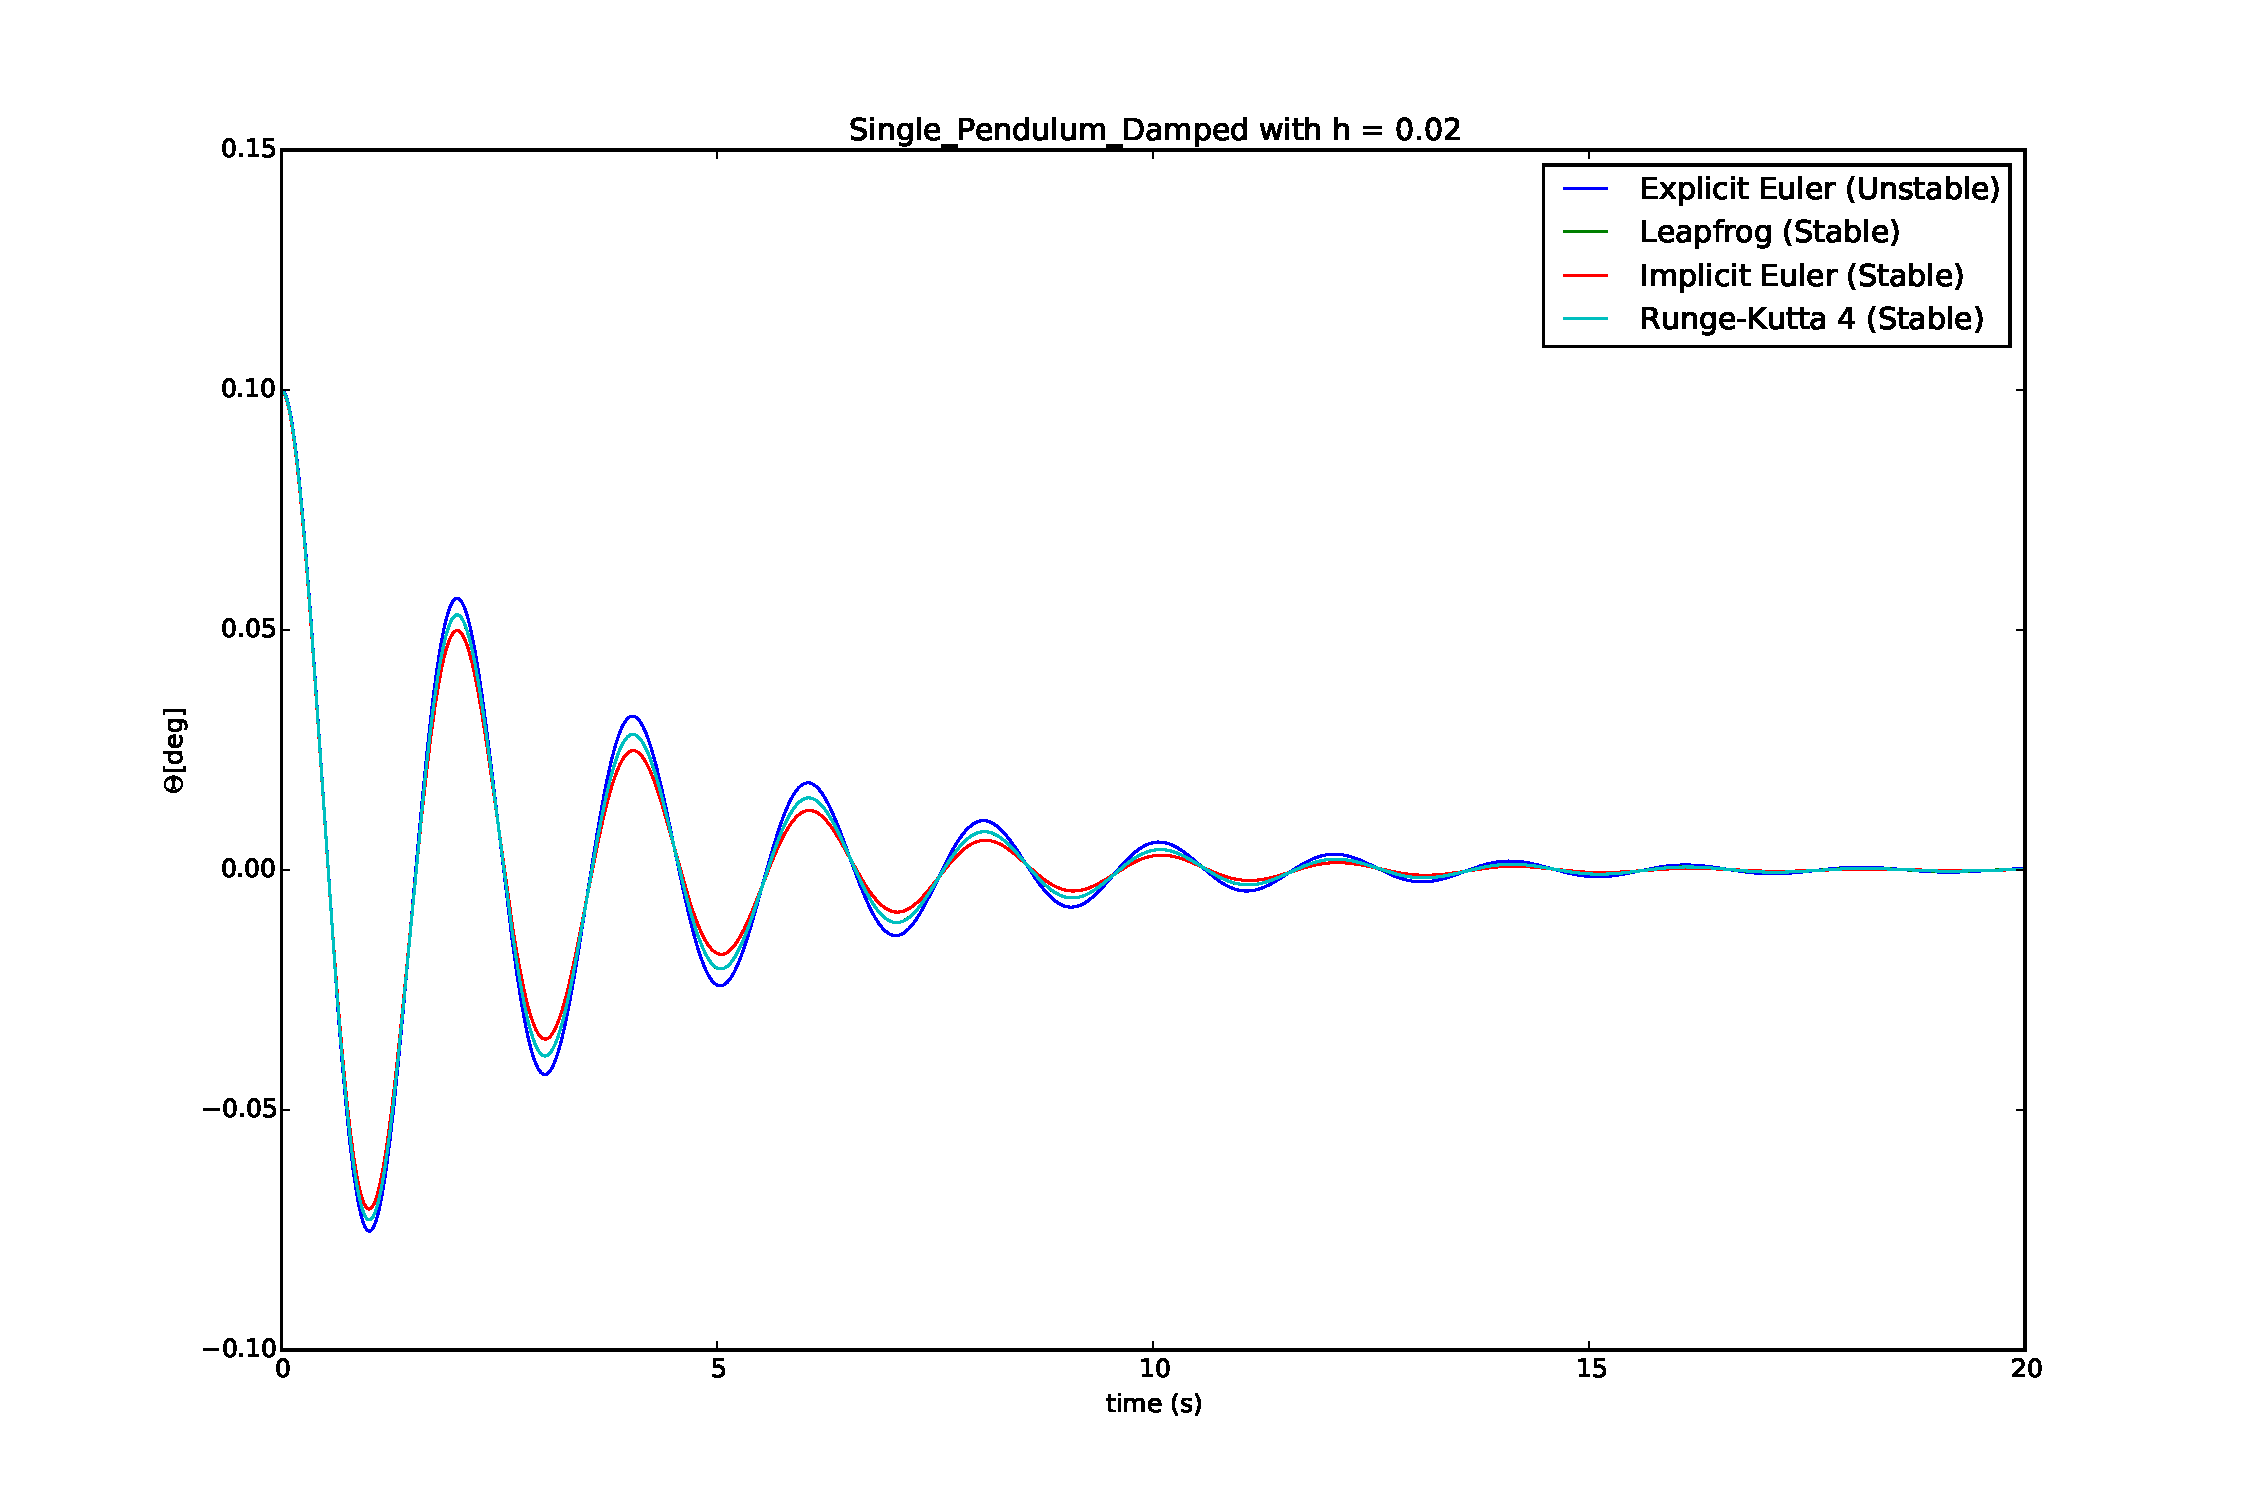
\includegraphics[width=0.9\textwidth]{Single_Pendulum_Damped_Theta}
\caption{The solutions for a damped single pendulum with $\hat{D}=0.2$. }
\label{fig:singledampedtheta}
\end{center}
\end{figure}

To determine stability thresholds, an initial stepsize of h=0.1 was used. An iterative testing process was used to estimate the threshold for stability, with $h_{i} = 1.02  \times h_{i-1}$ if the system was initially stable or $h_{i} =0.98 \times h_{i-1}$ if not. The threshold for stability are summarised in Table \ref{tab:stability}. Each threshold value has an associated error of approximately $\pm1\%$. The smallest tested threshold stepsize was 0.001, below which we leave the threshold undetermined.

\begin{table}[h!]
  \centering
  \caption{Threshold h value for stable solutions}
  \label{tab:stability}
  \begin{tabular}{ccc}
    \toprule
    Method & Undamped & Damped\\
    \midrule
     Explicit Euler & \textless 0.001 & $0.009 \pm 0.000$ \\
     Leapfrog & $0.174 \pm 0.002$ & $0.038\pm 0.000$\\
     Implicit Euler & $1.014 \pm 0.010$ & $1.165 \pm 0.016$\\
     Runge-Kutta 4 & $2.841 \pm 0.028$ & $3.015 \pm 0.030$\\
    \bottomrule
  \end{tabular}
\end{table}

\subsection{Arbitrary Amplitude Oscillations}
The simulation also works with a large oscillation angle such as $\theta_{0} = \frac{3}{4} \pi$. However, these energies are close to the maximum allowed $E_{max} = 2mgl_{1}$. If the pendulum energy exceeds this value, then it completes entire revolutions of the pivot point without stopping. This only occurs without the small angle approximation, using $\sin(\theta) \leq 1$ rather than the freely varying variable $\theta$. Use of the small angle approximation with the large $\theta_{0}$ leads to oscillations in the system energy, illustrated in Figure \ref{fig:badenergy}. The GPE is still calculated correctly, but the amplitude of KE oscillations are excessively large. This is due to the modelling of gravitational acceleration as proportional to $\theta$. Thus, at the given $\theta_{0}$, the gravitational acceleration will be $g\theta_{0} \approx 2.09g$ rather than the realistic $g\sin(\theta_{0}) \approx 0.71g$. The resultant velocities will all be too large, leading to excess KE. The small angle approximation is consequently not employed in the code.

\begin{figure}
\begin{center}
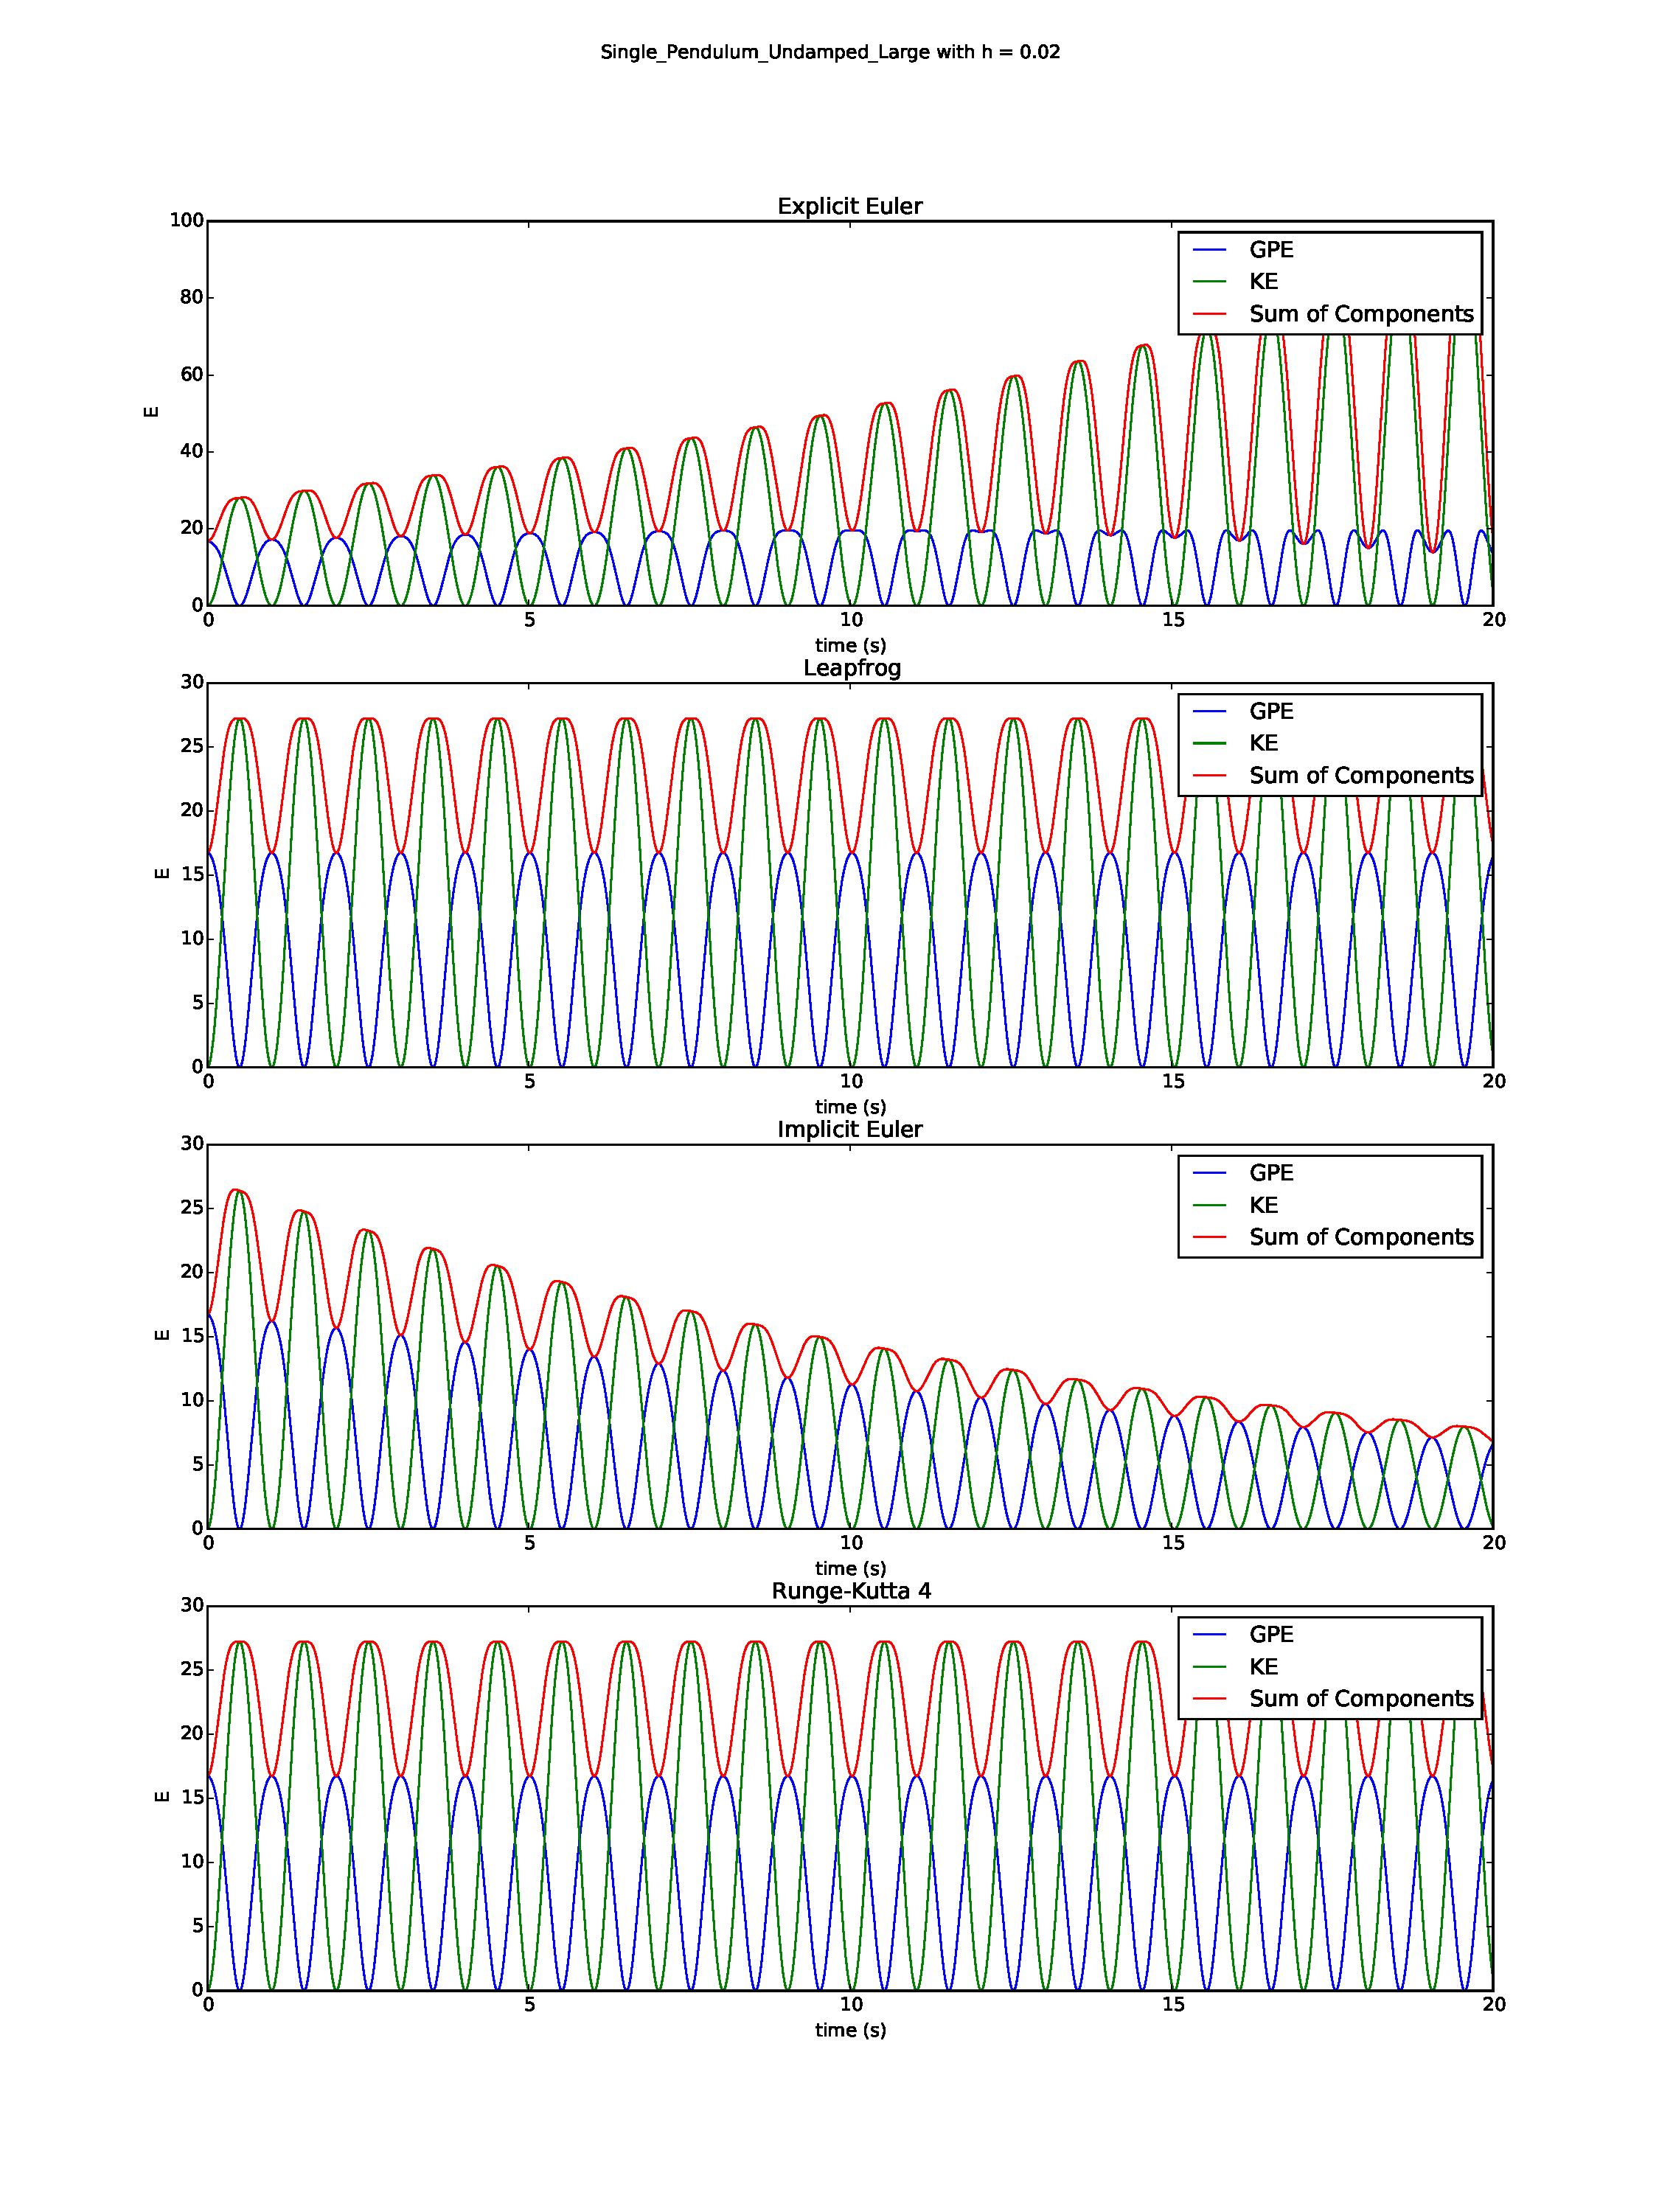
\includegraphics[width=0.9\textwidth]{Bad_Energy}
\caption{The components of Energy for the undamped single pendulum, with $\hat{D}=0$ and $\theta_{0} = \frac{3}{4} \pi$, when the small angle approximation is employed. The GPE continues to be calculated correctly, but the KE is overestimated due to an unrealistically large acceleration by gravity. As the Implicit Euler Solution decays, the solution converges on the true solution as the small angle approximation becomes more valid.}
\label{fig:badenergy}
\end{center}
\end{figure}

The stability of FDM solutions with a large $\theta_{0}$ depend again on the stepsize chosen. For a stepsize of h=0.02, the Explicit Euler FDM produced a stable damped solution but an unstable undamped solution. In the undamped case, that the pendulum gains energy with each revolution. Thus, the rotational frequency of the pendulum continuously increases. There is an exponential increase in the absolute value of the angle $\theta$, with the sign determined by the original direction of rotation at the time when the pendulum energy exceeded $E_{max}$. This is illustrated in Figure
\ref{fig:singledampedbigtheta}. 
\begin{figure}
\begin{center}
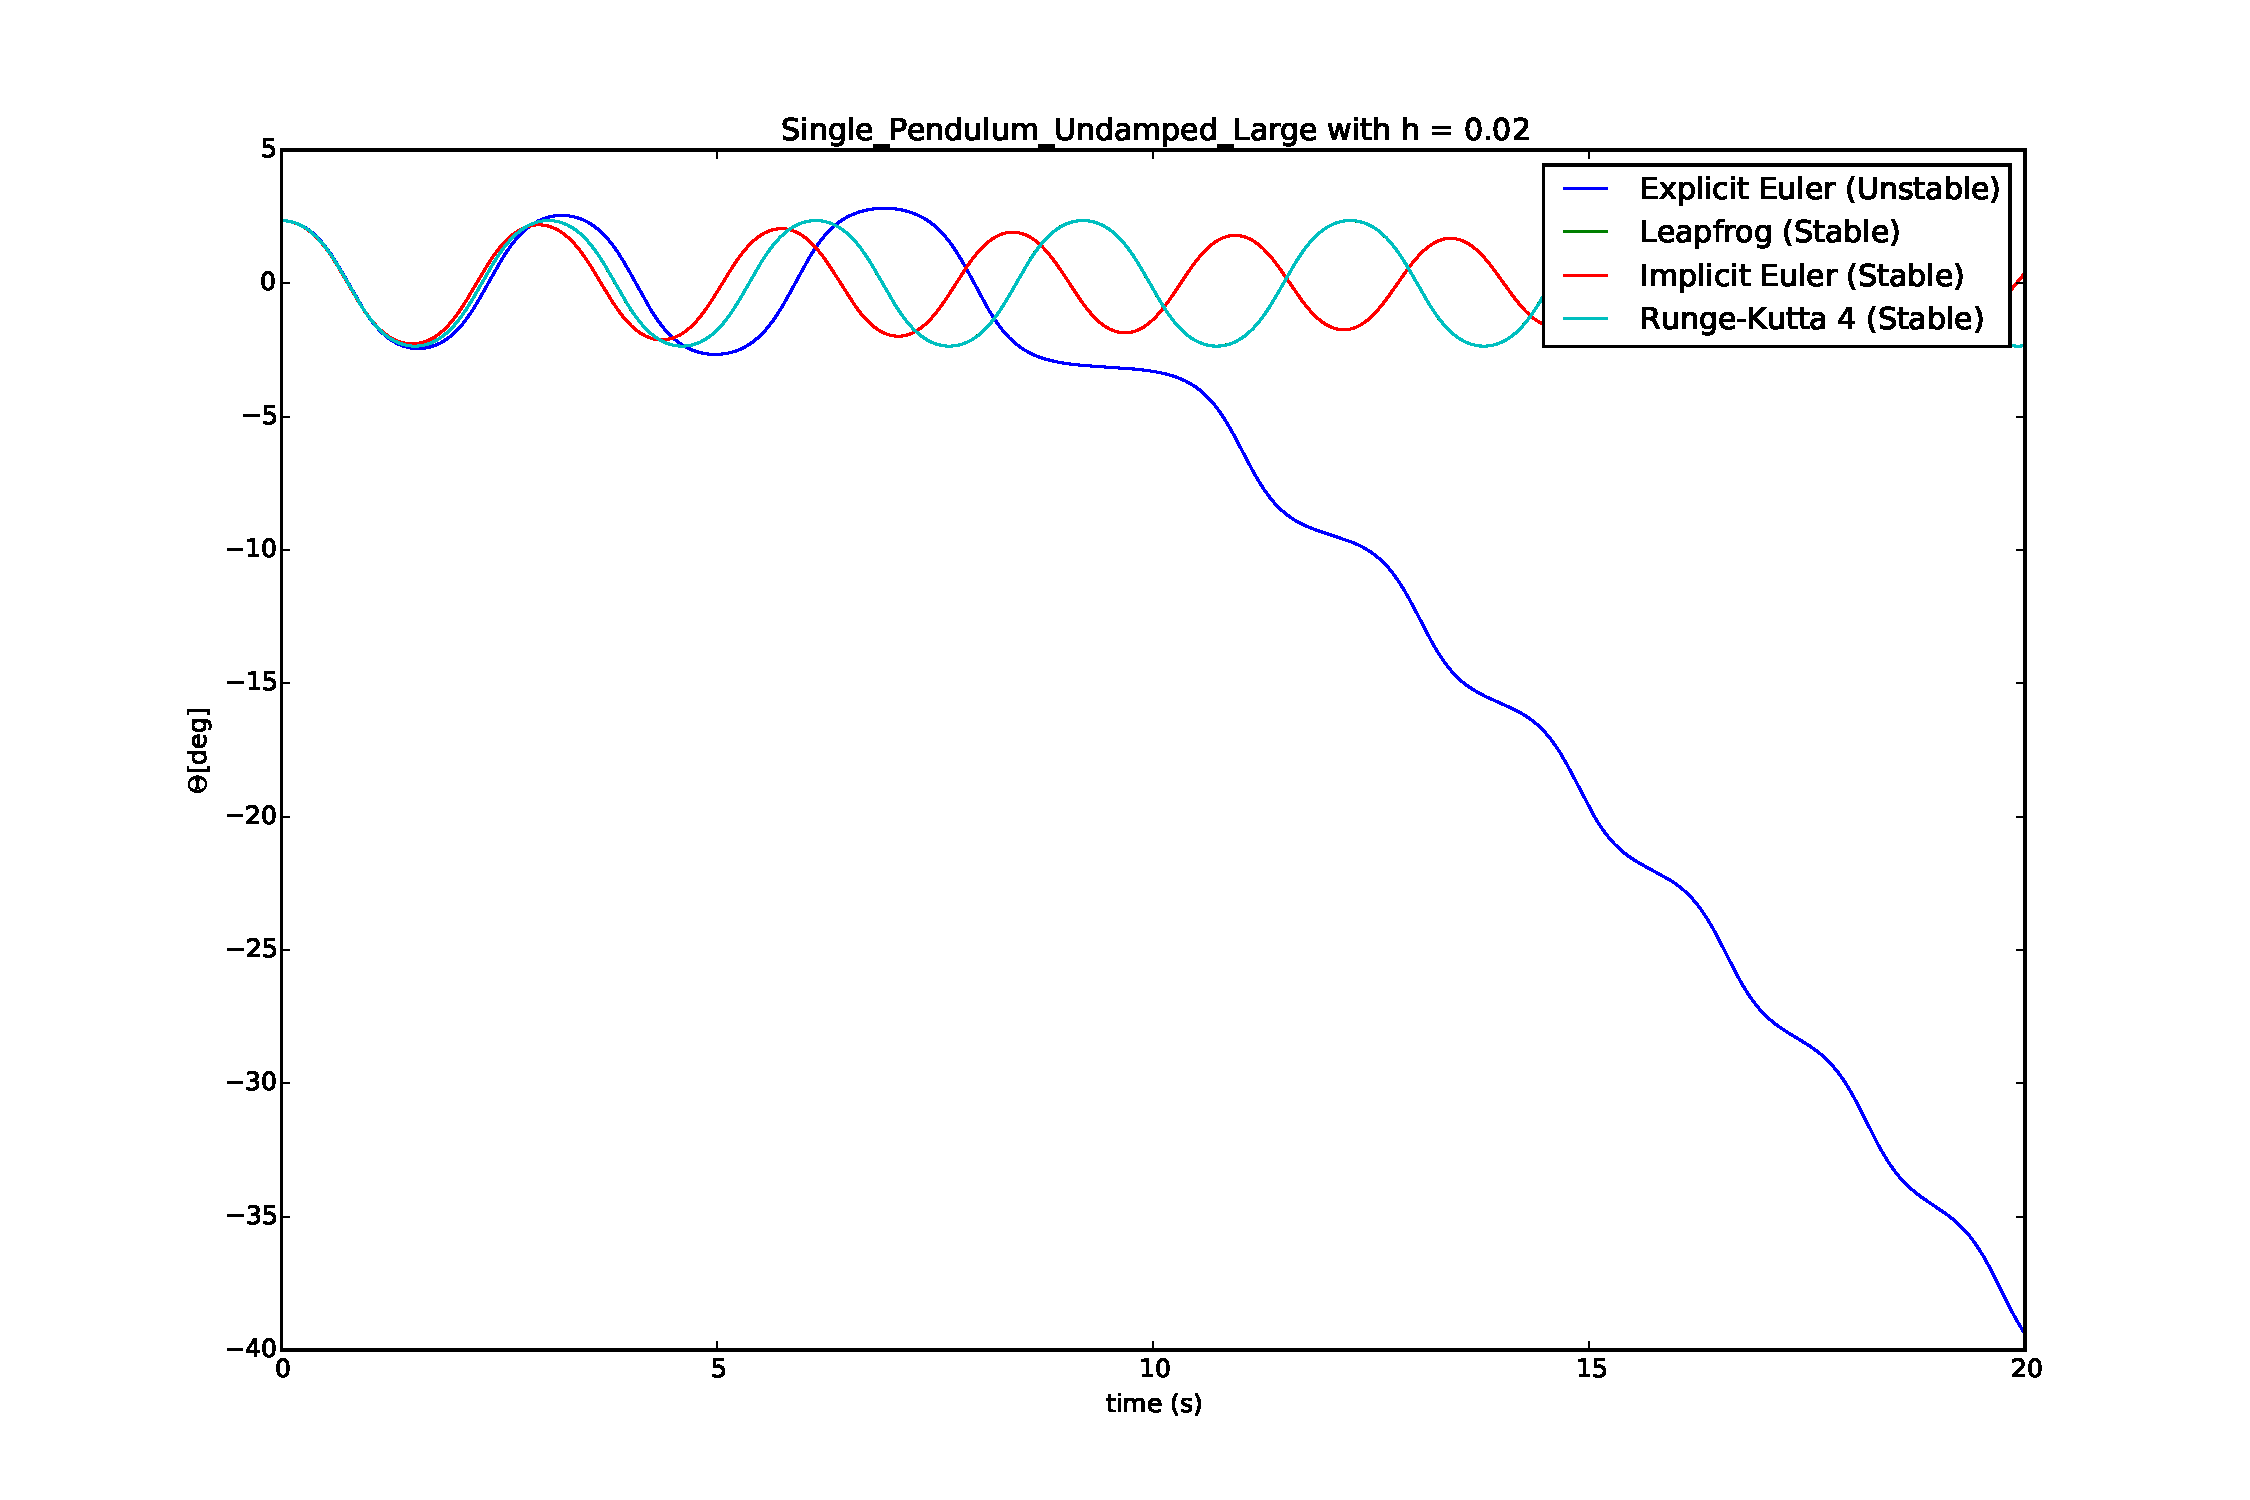
\includegraphics[width=0.9\textwidth]{Single_Pendulum_Undamped_Large_Theta}
\caption{The solutions for an undamped single pendulum with $\hat{D}=0.2$ and $\theta_{0} = \frac{3}{4} \pi$. Due to the increasing system energy, the Explicit Euler pendulum completes full rotations about the pivot.}
\label{fig:singledampedbigtheta}
\end{center}
\end{figure}

Considering the qualitative observations of FDM behaviour, the results in Table \ref{tab:stability}, and the continued stability even with large undamped oscillations, it is clear that the Runge-Kutta 4 method is the best numerical method for a flexible simulation. It was the only method to perform reliably in both damped and undamped oscillating motion, as well as being the most stableand fastest-converging method. This is at the expense of raw computational processing time per step, due to the four derivative calculations per step in comparison to one or two for the other methods.
 
\section{Double Pendulum}
The chaotic nature of double pendulum systems is much more challenging for FDMs. In addition to a new equation of motion for the second pendulum, we must also modify the equation of motion for the first pendulum and solve two additional coupled equations. We introduce the variable $\phi$, defined as the angle between the second pendulum and the vertical. For a second pendulum of mass $m_{2}$, we have the equations of motion:

\[ \frac{d^{2}\theta}{dt^{2}} = - \frac{g}{l_{1}} \sin(\theta) + \frac{m_{2}g}{m_{1}l_{1}}\sin(\phi-\theta)- \frac{D}{m_{1}l_{1}} \frac{d\theta}{dt} \]
\[ \frac{d^{2}\phi}{dt^{2}} + \frac{d^{2}\theta}{dt^{2}}= - \frac{g}{l_{2}} \sin(\phi) - \frac{D}{m_{2}l_{2}} (\frac{d\theta}{dt} + \frac{d\phi}{dt})\]

The derivation of four dimensionless coupled equations, as well as the system energy, is described in the Appendix. The total system energy is the sum of both pendulum energies.

\subsection{Parameter Variation}
We can consider three general cases for simulation, defined by the ratio $R=\frac{m_{2}}{m_{1}}$. We have the small-R (R=0.01), equal-R (R=1) and big-R (R=100) cases, with significant variation in behaviour. The breakdown of energy into components, is seen in Figure \ref{fig:doubleundampedenergy}. 

For small-R, there is obvious interference between the independent oscillating modes of each pendulum. Consequently the system energy oscillates between the two pendulums. The individual motion of each pendulum is roughly that of a single pendulum with varying total energy. When damped, both pendulums quickly moves to rest.

For equal-R, the energy chaotically passes between the two pendulums, though the second pendulum is never at rest. In effect, there is a floor on the energy of pendulum two and a ceiling on the energy of pendulum 1. The relative GPE and KE components also vary chaotically. When damped, the heavy first pendulum quickly moves to rest, while the lighter second pendulum does so at a much slower rate.

For big-R, the sum of angles $\theta$ and $\phi$ oscillates slowly as the heavy second pendulum moves. In addition, the individual values for $\theta$ and $\phi$ oscillate quickly around the sum, as the first pendulum oscillates almost freely between the pivot and almost-fixed second mass. The energy division between the two pendulums oscillates rapidly between the two extremes of equal division and all energy in the heavy second pendulum. When damped, the fast-oscillating first pendulum is quickly slowed until $\omega = \nu$, leaving the system to oscillate like a single pendulum.

\begin{figure}
\begin{center}
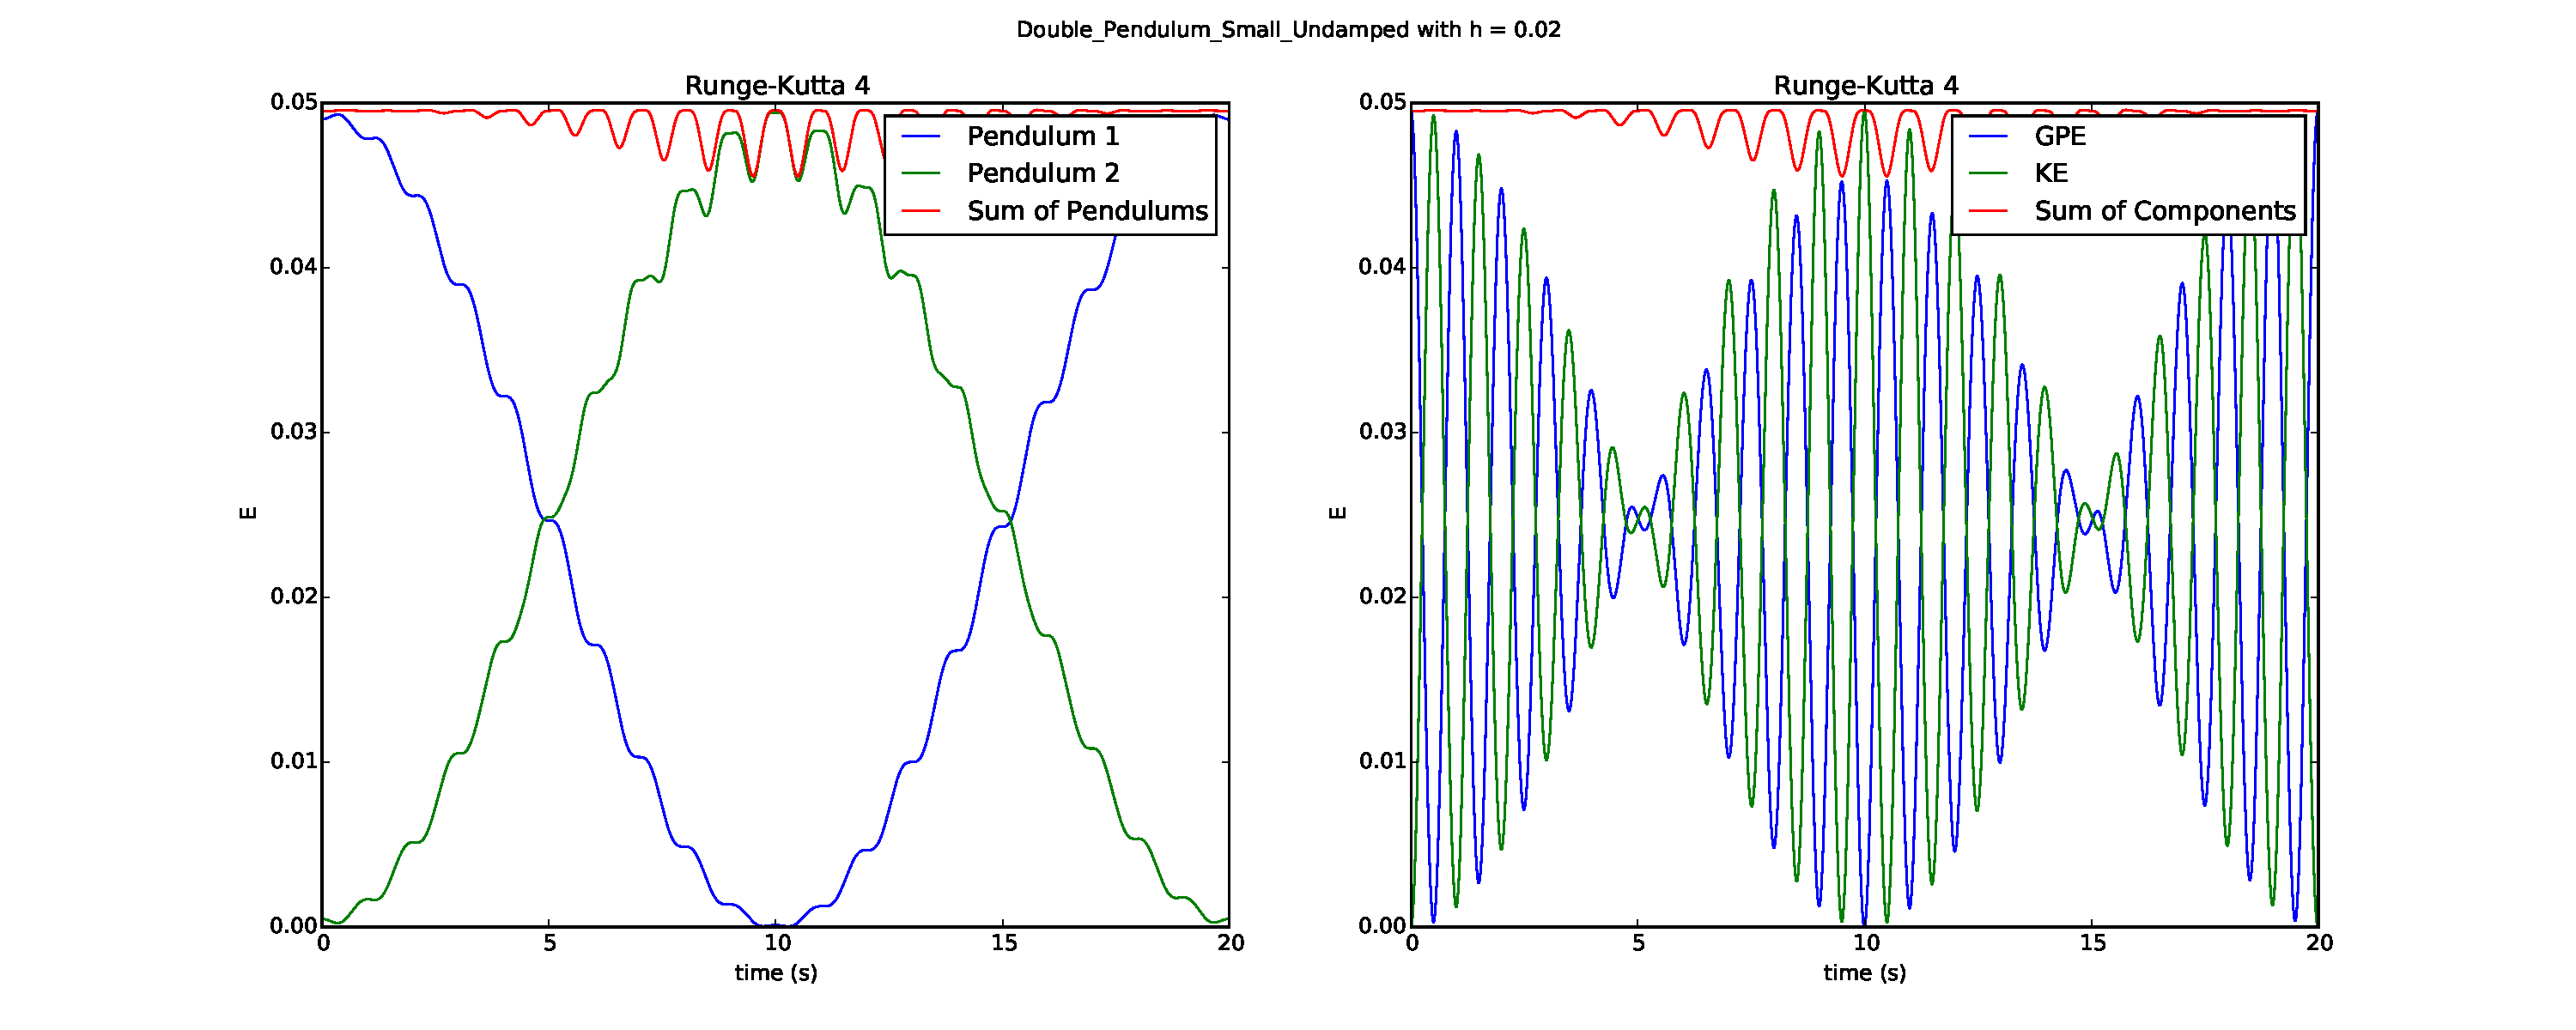
\includegraphics[width=0.9\textwidth]{Double_Pendulum_Small_Undamped_Energy_Components}
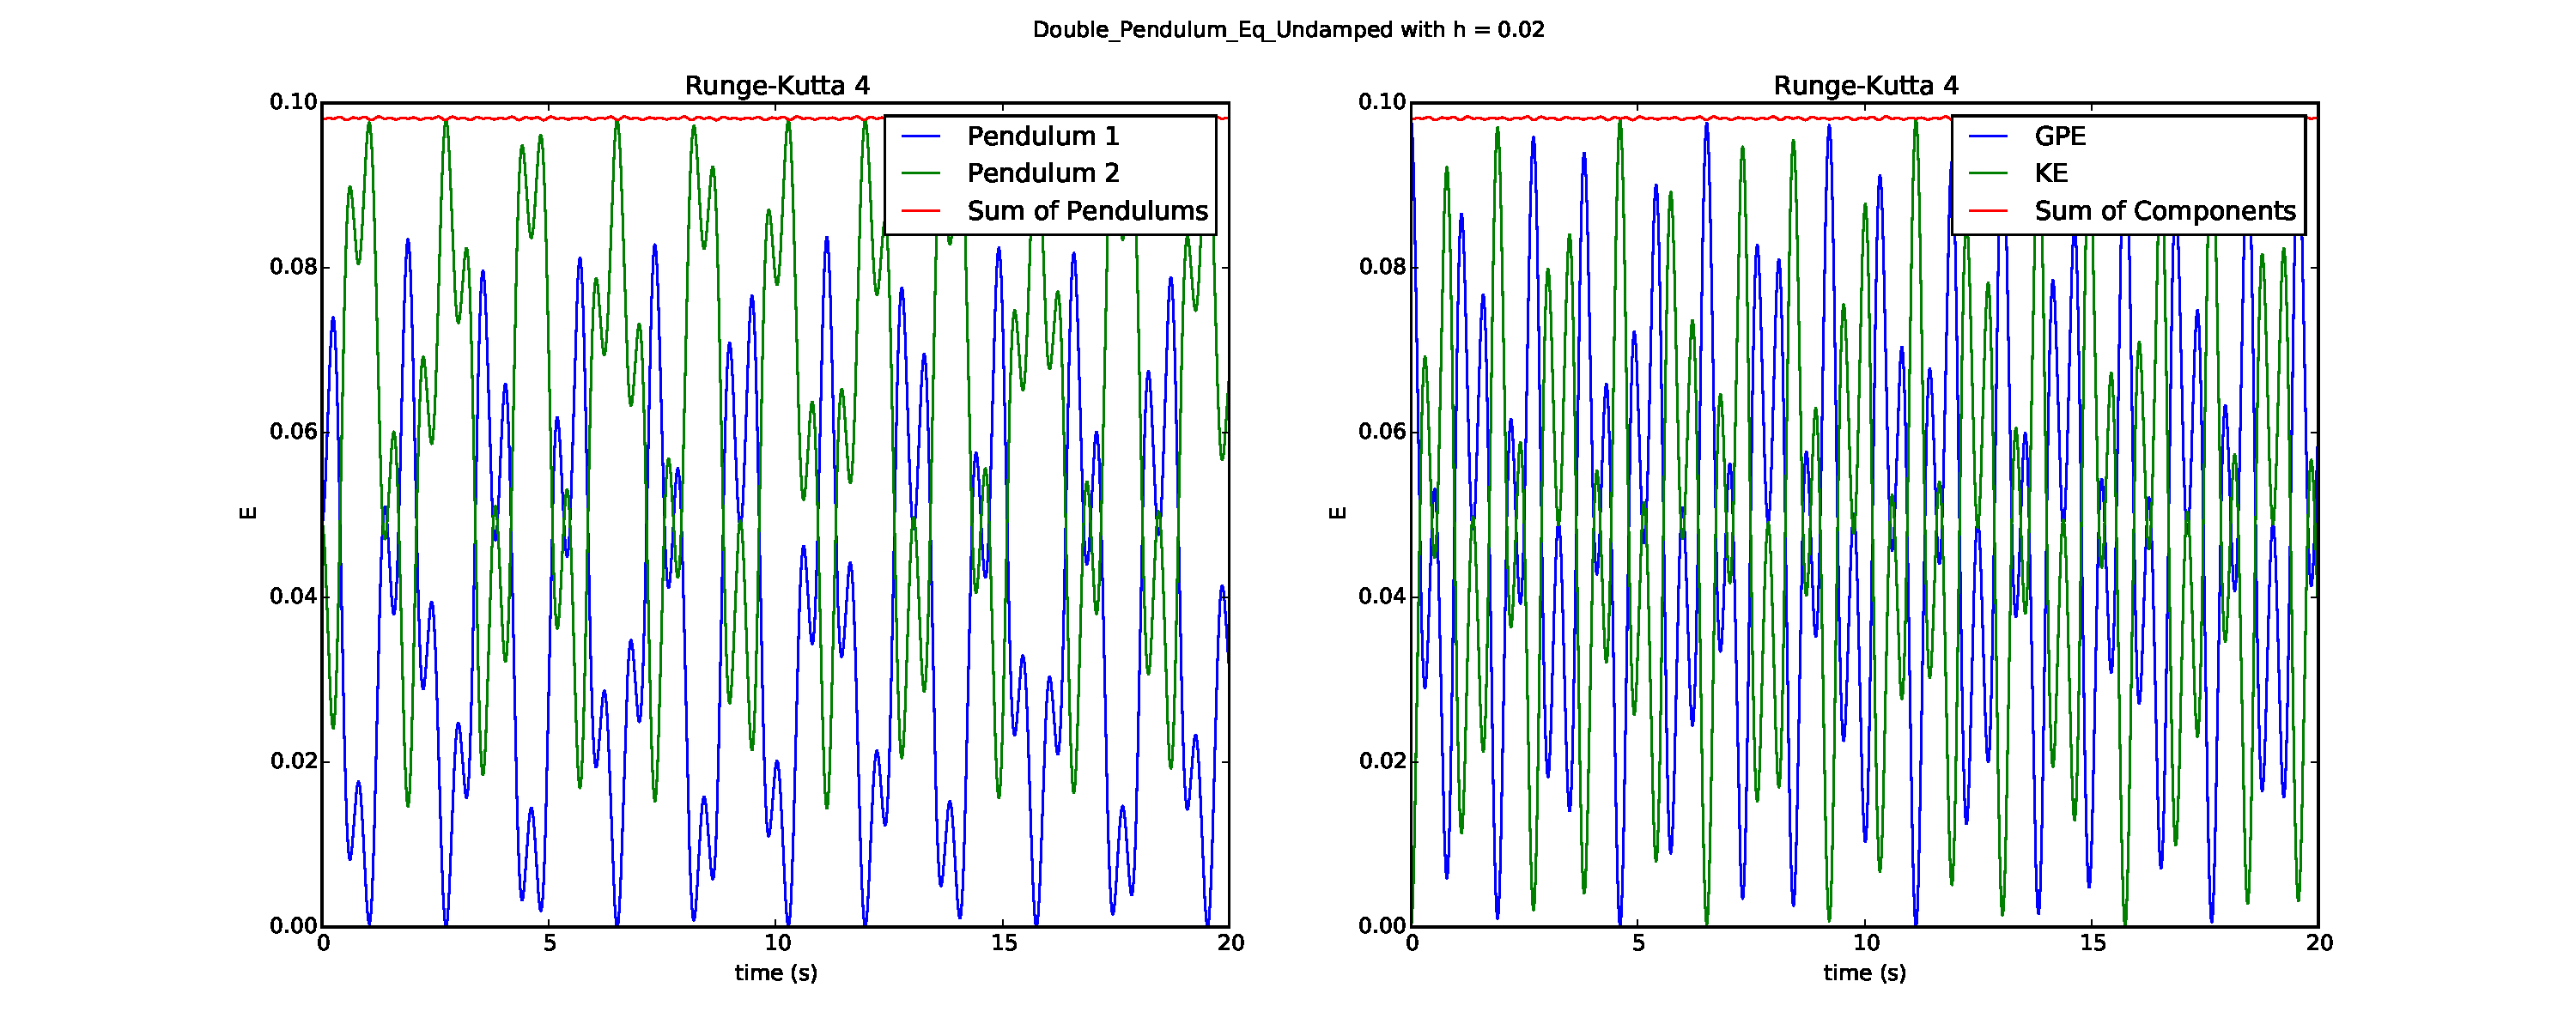
\includegraphics[width=0.9\textwidth]{Double_Pendulum_Eq_Undamped_Energy_Components}
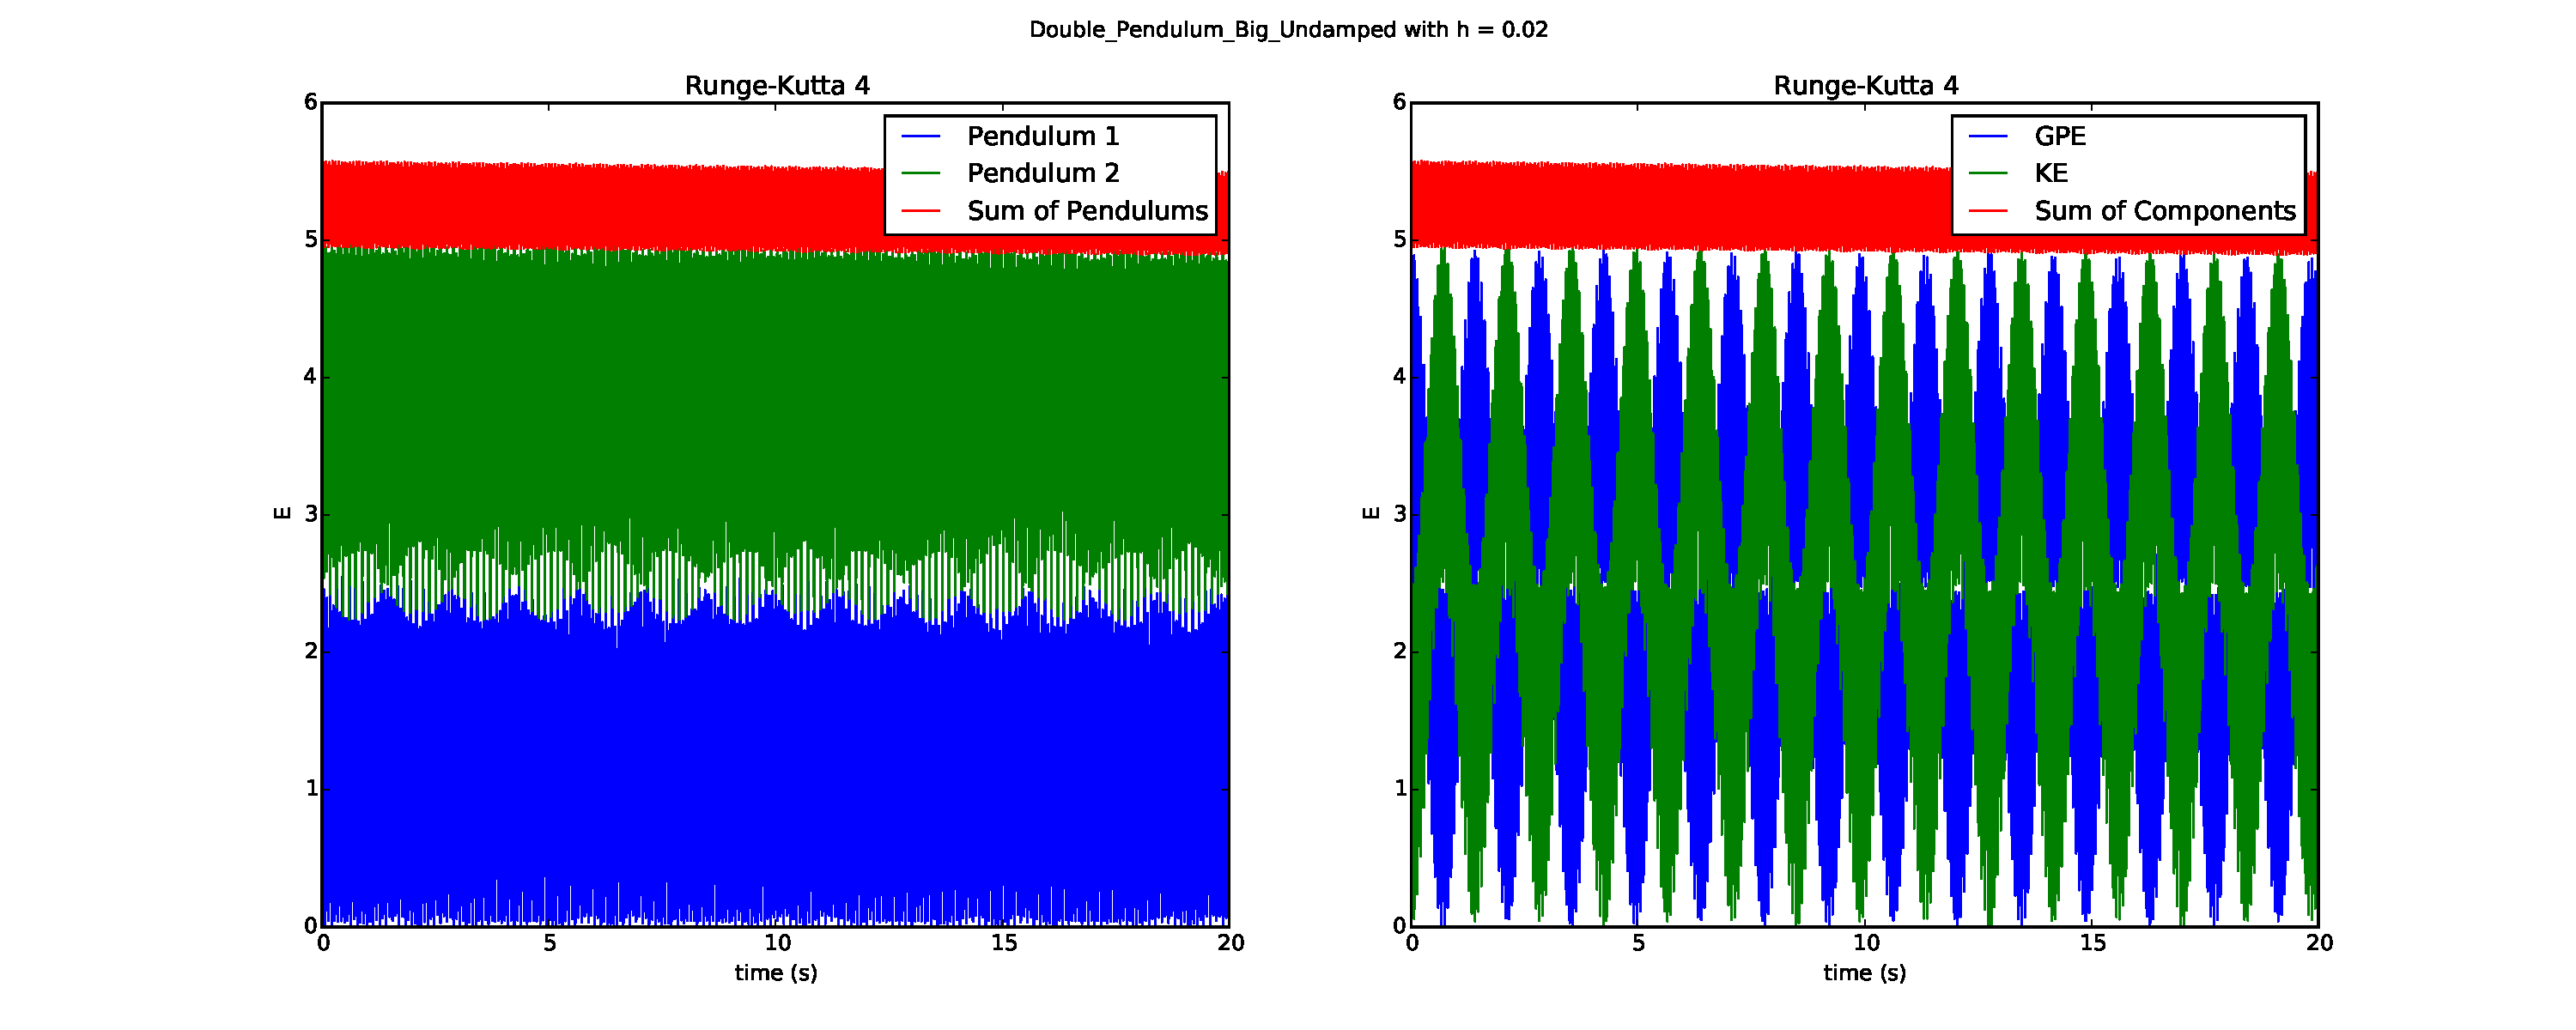
\includegraphics[width=0.9\textwidth]{Double_Pendulum_Big_Undamped_Energy_Components}
\caption{The energy components for an undamped double pendulum oscillations with $\hat{G}=1.0$ and $\theta_{0} = 0.1$. All three solutions appear roughly stable. The small-R solution represents energy oscillating between the two pendulums. The equal-R solution indicates chaotic coupling. The big-R solution shows a superposition of independent heavy-pendulum and light-pendulum oscillations.}
\label{fig:doubleundampedenergy}
\end{center}
\end{figure}

Strictly speaking, all undamped solutions are unstable. However, the total energy of each system does oscillate around value that appears to be constant, so they would be better described as \textquoteleft Approximately Stable'. The big-R solution has the largest energy oscillation. In the damped case, both small-R and equal-R damped solutions are stable. With h=0.02, the big-R case is still \textquoteleft Approximately Stable', though with a clear decrease in system energy over time rather than appearing to remain constant. This instability in the damped big-R system is caused by an initial increase in System Energy. In general, the system energy was most reliable calculated when $R\approx 1$.

\begin{figure}
\begin{center}
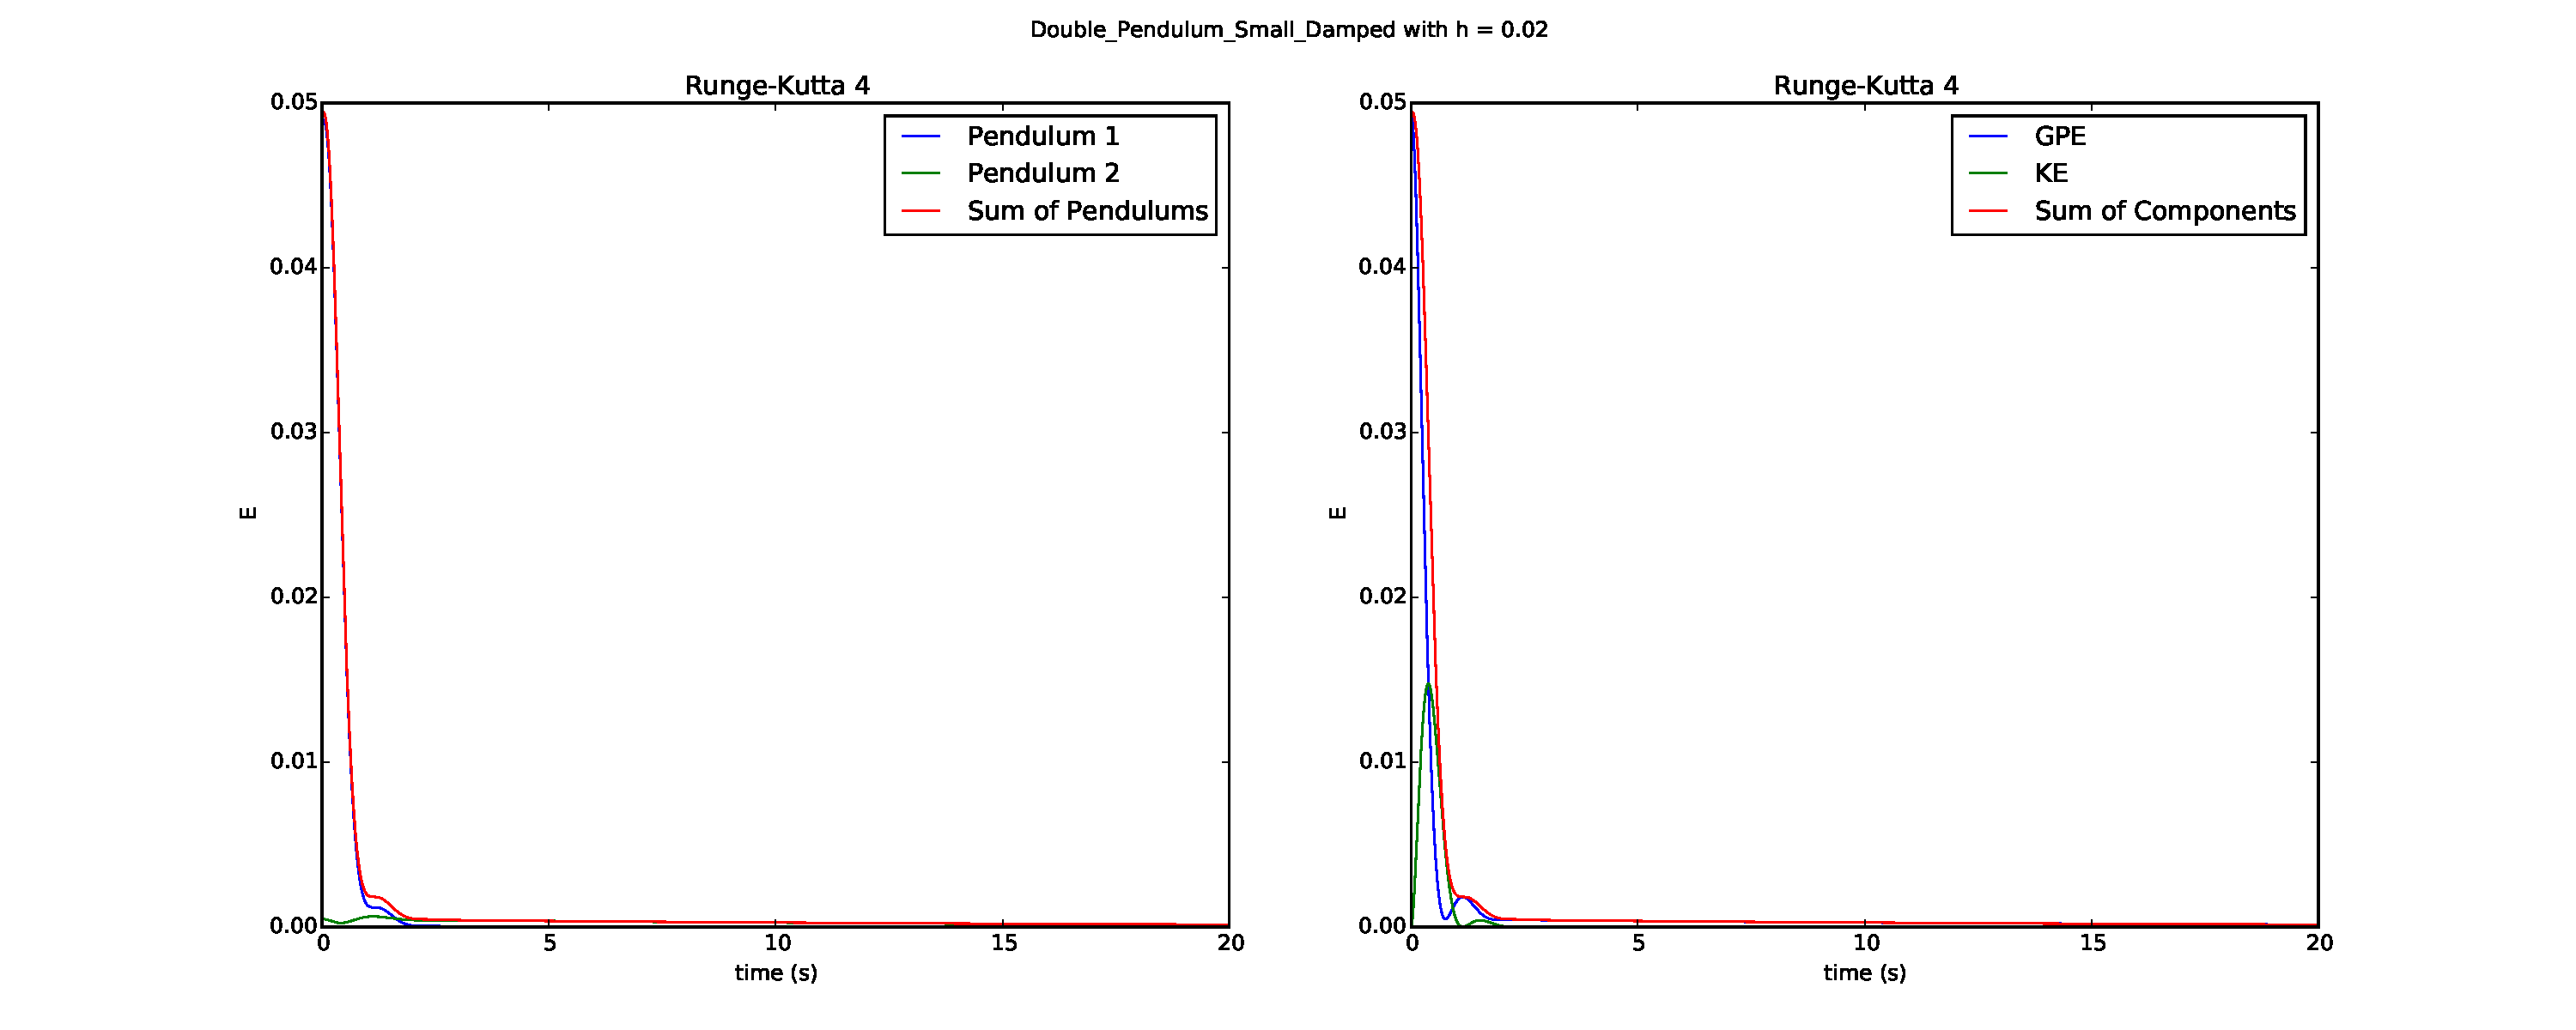
\includegraphics[width=0.9\textwidth]{Double_Pendulum_Small_Damped_Energy_Components}
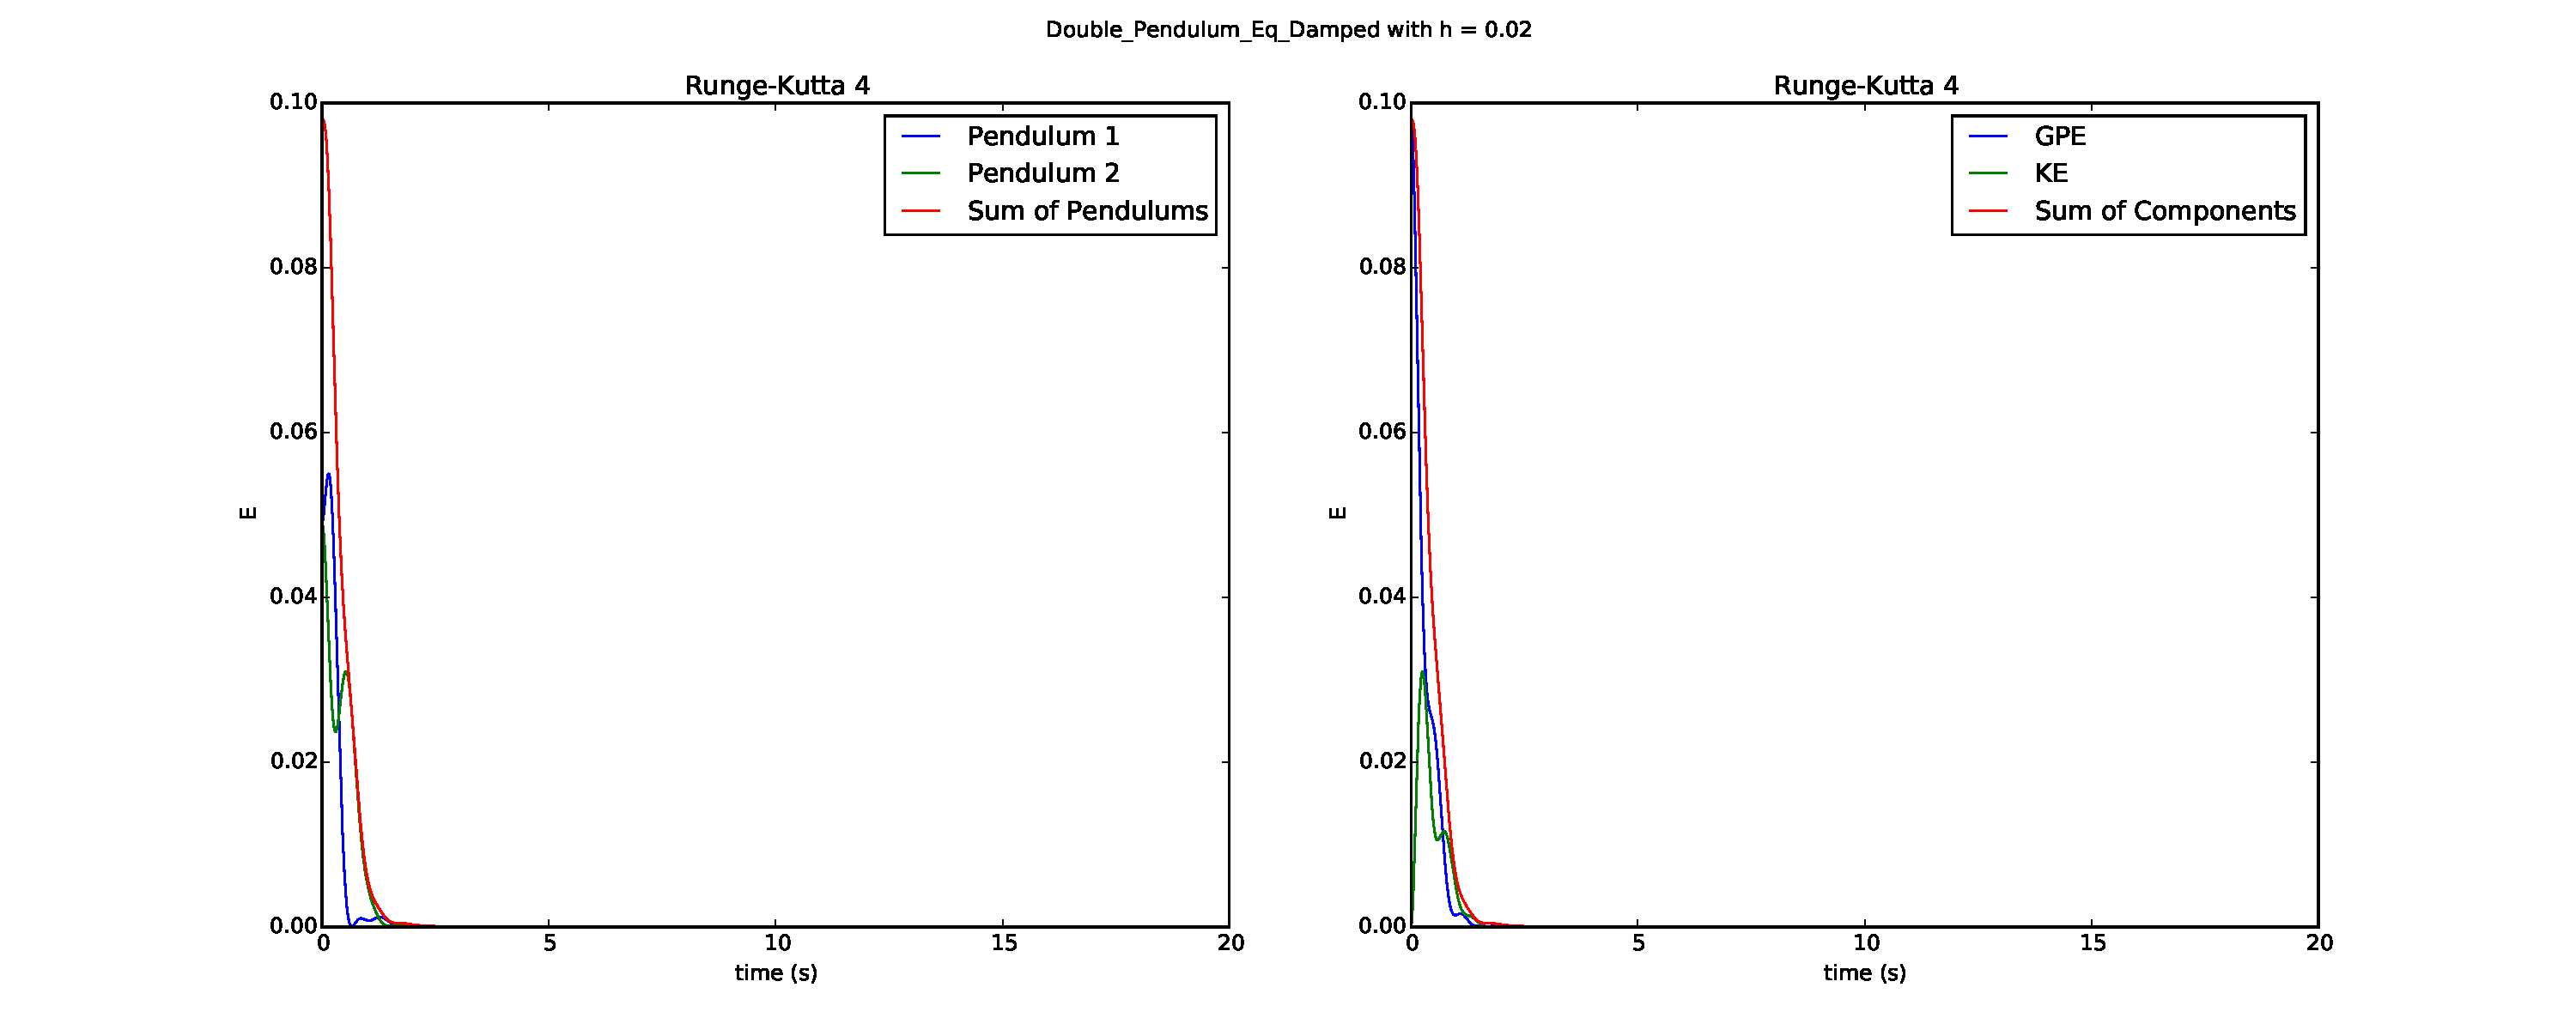
\includegraphics[width=0.9\textwidth]{Double_Pendulum_Eq_Damped_Energy_Components}
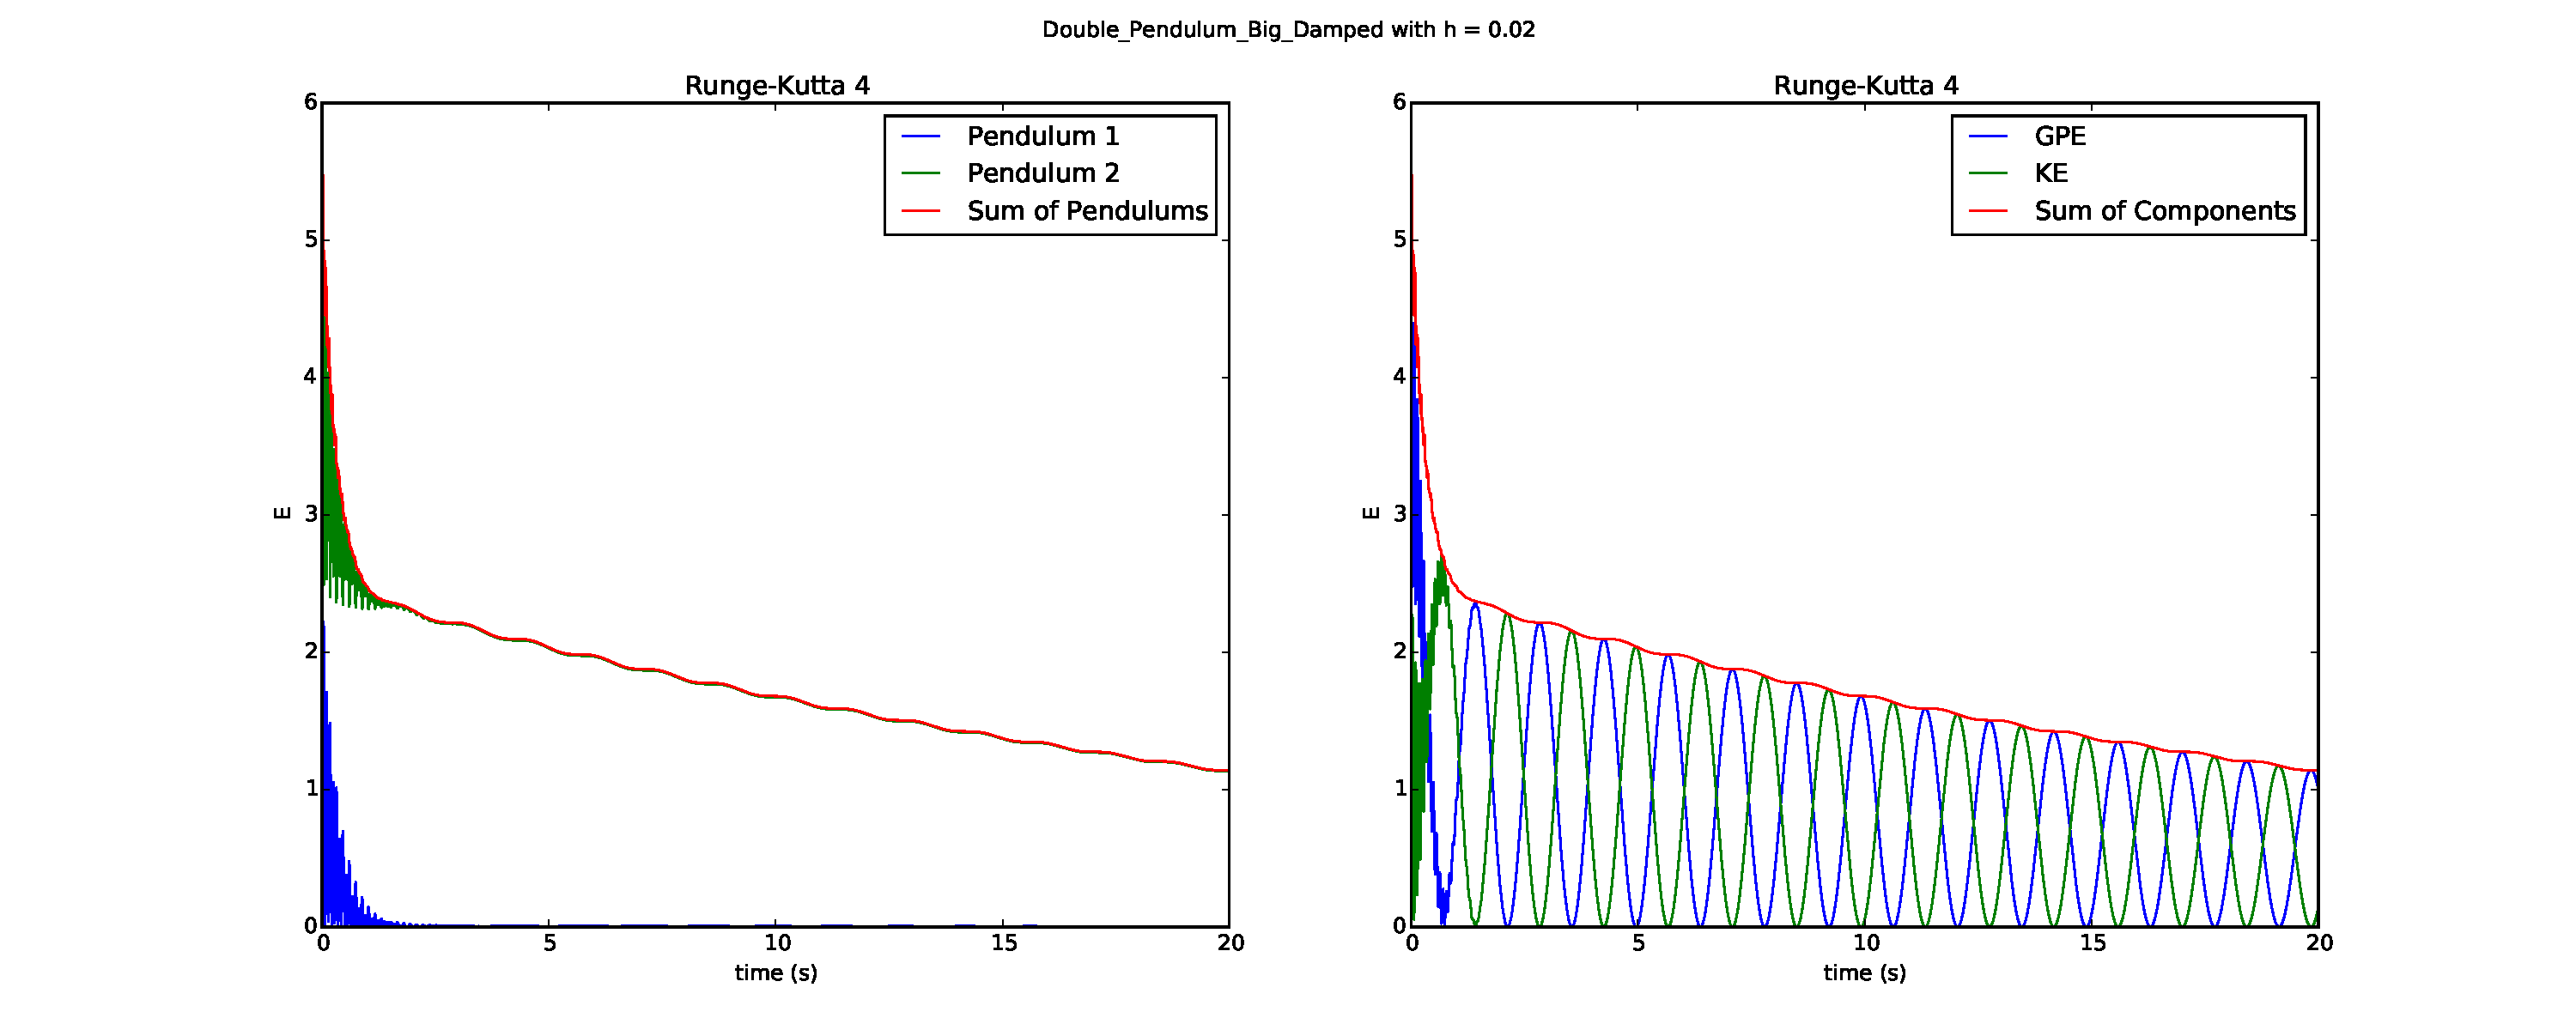
\includegraphics[width=0.9\textwidth]{Double_Pendulum_Big_Damped_Energy_Components}
\caption{The energy components for a damped double pendulum oscillations with $\hat{G}=1.0$ and $\theta_{0} = 0.1$. Both the small-R and equal-R solutions decay rapidly to rest. The big-R solution quickly decays into a single pendulum solution.}
\label{fig:doubledampedenergy}
\end{center}
\end{figure}

\section{Conclusion}
Initially, a simple single pendulum was simulated to explore the stability of various FDMs. It was found that, across many measures, the Runge-Kutta 4 method was superior. This method was then applied to a double pendulum system. It was found that for an undamped double pendulum could not be accurately simulated. However, solutions could be considered \textquoteleft Approximately Stable', and still gave a clear indication of the physical motion in each case. Heavily damped systems were found to be simulated in a more stable way. Ultimately, the stability decreased as $\log(R)$ moved from a value of 0. A dynamic stepsize could be calculated with reference to the quantity $\log(R)$, to account for this.

(Word Count $\approx$ 2000)

\section{Appendix}
\subsection{Finite Differential Methods}
For each FDM, we are required to know the inital value of the variable y. In addition, we require knowledge of the function $f(y) = \frac{dy}{dt}$. Then, for a stepsize h, we can calculate the next step in the series solution. In the case of multivariate functions, we simply replace the variable y with the vector \textbf{y}, containing each variable. We then perform the FDM on each variable simultaneously.
\subsubsection{Explicit Euler}
For the Explicit Euler Method, we define the next step in the following way:

\[ \Delta_{y} = f(y_{i-1}) \]
\[ y_{i} = y_{i-1} + (h \times \Delta_{y}) \]

\subsubsection{Leapfrog Method}
For the Leapfrog Method:

\[ \Delta_{y} = f(y_{i-1}) \]
\[ y_{i} = y_{i-2} + (2 \times h \times \Delta_{y}) \]
\subsubsection{Runge-Kutta 4}
For the Runge-Kutta 4 Method:

\[ k_{1} = f(y_{i-1}) \]
\[ k_{2} = f(y_{i-1} + (k_{1} \times \frac{h}{2})) \]
\[ k_{3} = f(y_{i-1} + (k_{2} \times \frac{h}{2})) \]
\[ k_{4} = f(y_{i-1} + (k_{3} \times h)) \]
\[ y_{i} = y_{i-1} + (\frac{k_{1} + 2(k_{2} + k_{3}) + k_{4}}{6} \times h) \]
\subsubsection{Implicit Euler}
For the Implicit Euler Method:

\[ y_{guess} = y_{i-1} + (h \times f(y)) \]
\[ \Delta_{y} = f(y_{guess}) \]
\[ y_{i} = y_{i-1} + (h \times \Delta_{y}) \]
\subsection{Single Pendulum Mathematics}
We can rescale the equation of motion for a single pendulum to make a dimensionless pair of coupled equations, with $\hat{t} = a t$ and $\hat{D} = b D$. Then we obtain two equations for variable evolution:

\[ \frac{d\theta}{d\hat{t}} = \omega \]
\[ \frac{d^{2}\theta}{d\hat{t}^{2}} = -\sin(\theta) - \hat{D} \omega \]
with the resultant values constants $a = \sqrt{\frac{g}{l}}$ and $b =m_{1}\sqrt{gl}$. Using an FDM, the values of the two variables $\theta$ and $\omega$ can be calculated for each step with reference to the previous variable values and the two equations above. 

The total energy of the system can then be calculated with reference to the component Kinetic Energy (KE) and Gravitational Potential Energy (GPE). For a pendulum of length $l_{1}$, we have:

\[ KE = \frac{1}{2}m_{1} v_{1}^{2} \]
\[ GPE = m_{1} * g * (y_{1} - l_{1}) \]
The system will thus have an energy of 0 when at rest. We can calculate the velocity of the single pendulum with reference to its position. We know that:
\[ x_{1} = l \sin(\theta) \]
\[ y_{1} = -l \cos(\theta) \]
It is simple to differentiate these definitions to find expressions for the velocity components:
\[ v_{1x} = \frac{dx}{dt} = l_{1} \frac{d\sin(\theta)}{dt} = l_{1} \frac{d\sin(\theta)}{d\theta} \frac{d\theta}{dt} = l_{1} \cos(\theta) \frac{d\theta}{dt}\]
\[ v_{1y} = \frac{dy}{dt} = -l_{1} \frac{d\cos(\theta)}{dt} = -l_{1} \frac{d\cos(\theta)}{d\theta} \frac{d\theta}{dt} = l_{1} \sin(\theta) \frac{d\theta}{dt}\]
It is thus clear to see that:
\[ v_{1}^2 = v_{1x}^2 + v_{1y}^2 = l_{1}^2 (\frac{d\theta}{dt})^2(\sin^2(\theta) + \cos^2(\theta)) = l_{1}^2 (\frac{d\theta}{dt})^2\]
\[ v_{1} = l_{1} \frac{d\theta}{dt} = a l_{1} \omega \]
This derivation is trivial for the case of the single pendulum, but the values of components $v_{1x}$ and $v_{1y}$ will be important for application to calculation of the double pendulum velocity.

\subsection{Double Pendulum Mathematics}
We can analogously transform the Double Pendulum equations of motion with the assumption $l_{1}=l_{2}=l$ yielding four dimensionless equations:

\[ \frac{d\theta}{d\hat{t}} = \omega \]
\[ \frac{d^{2}\theta}{d\hat{t}^{2}} = - \sin(\theta) + R\sin(\phi-\theta)- \hat{G} \omega \]
\[ \frac{d\phi}{d\hat{t}} = \nu \]
\[ \frac{d^{2}\phi}{d\hat{t}^{2}} = -\sin(\phi) - \frac{\hat{G}}{R} (\omega + \nu) - \frac{d^{2}\theta}{d\hat{t}^{2}}\]
Again $a = \sqrt{\frac{g}{l}}$, but here $G =\frac{D}{m_{1}\sqrt{gl}}$ and $R=\frac{m_{2}}{m_{1}}$.
The Double Pendulum Energy can be calculated with reference to the component Kinetic Energy (KE) and Gravitational Potential Energy (GPE). The energy of the first pendulum is calculated in an identical way to the single pendulum system. For a second pendulum of length $l_{2}$, we have:

\[ KE = \frac{1}{2}m_{2} v_{2}^{2} \]
\[ GPE = m _{2}* g * (y_{2} - (l_{1}+l_{2})) \]
A sum of both pendulum energies yields the total system energy. The system will again have an energy of 0 when at rest. 

It is most instructive to think of the motion of the second pendulum as a superposition of two motions. The first is the motion $v_{2, pivot}$ of the pivot point, assuming the second pendulum were to remain motionless. The other motion $v_{2, pen}$ to consider is that of the second pendulum in relation to its pivot point, assuming the pivot point is stationary. 

It is in fact easy to calculate the velocity $v_{2, pivot}$, because we know that the pivot point of the second pendulum is simply the first pendulum. Thus $v_{2, pivot} = v{1}$. Then, in analogous way to for a single pendulum, we find that:
 
\[ v_{2,pen,x} = l_{2} \cos(\phi) \frac{d\phi}{dt}\]
\[ v_{2, pen,y} = l_{2} \sin(\phi) \frac{d\phi}{dt}\]

Thus, having calculated each component:
\[v_{2} = v_{1} + v_{2, pen}\]
\[ v_{2,x} = l_{1} \cos(\theta) \frac{d\theta}{dt} + l_{2} \cos(\phi) \frac{d\phi}{dt}\]
\[ v_{2,y} = l_{1} \sin(\theta) \frac{d\theta}{dt} + l_{2} \sin(\phi) \frac{d\phi}{dt}\]
\[v_{2} =\sqrt{v_{2,x}^{2} + v_{2,y}^{2}}\]

This simplifies velocity calculations greatly, because of the resultant general rule that: 
\[ v_{i,x} = v_{i-1, x}+ l_{i} \cos(\theta_{i}) \frac{d\theta_{i}}{dt} = v_{i-1, x}+ al\cos(\theta_{i})\omega_{i}\]
\[ v_{i,y} = v_{i-1, y}+ l_{i} \sin(\theta_{i}) \frac{d\theta_{i}}{dt}= v_{i-1, y} + al\sin(\theta_{i})\omega_{i}\]

The code made use of this generalisation to enable easy adaptability to n-pendulum systems. The same general rule applies to position coordinates:

\[ x_{i} = x_{i-1}+ l_{i} \sin(\theta_{i})\]
\[ y_{i} = y_{i-1} - l_{i} \cos(\theta_{i})\]
\end{document}